% Template for a Computer Science Tripos Part II project dissertation
\documentclass[12pt,a4paper,twoside,openright]{report}
\usepackage[pdfborder={0 0 0}]{hyperref}    % turns references into hyperlinks
\usepackage[margin=25mm]{geometry}  % adjusts page layout
\usepackage{graphicx}  % allows inclusion of PDF, PNG and JPG images
\usepackage{verbatim}
\usepackage{docmute}   % only needed to allow inclusion of proposal.tex
\usepackage{tabularx}
\usepackage{listings}
\usepackage[chapter]{minted}
\usepackage[english]{babel}
\usepackage{blindtext}
\usepackage{algorithm2e}

\lstset{
basicstyle=\small\ttfamily,
breaklines=true
}

% Ensures listing and lstlisting use the same counter.
\AtBeginEnvironment{listing}{\setcounter{listing}{\value{lstlisting}}}
\AtEndEnvironment{listing}{\stepcounter{lstlisting}}

\raggedbottom                           % try to avoid widows and orphans
\sloppy
\clubpenalty1000%
\widowpenalty1000%

\renewcommand{\baselinestretch}{1.1}    % adjust line spacing to make
                                        % more readable

\begin{document}

\bibliographystyle{plain}


%%%%%%%%%%%%%%%%%%%%%%%%%%%%%%%%%%%%%%%%%%%%%%%%%%%%%%%%%%%%%%%%%%%%%%%%
% Title


\pagestyle{empty}

\rightline{\LARGE \textbf{Jacob Fenton}}

\vspace*{60mm}
\begin{center}
\Huge
\textbf{Efficient Asymmetric Cryptography for RFID Access Control} \\[5mm]
Computer Science Tripos -- Part II \\[5mm]
Fitzwilliam College \\[5mm]
\today  % today's date
\end{center}

%%%%%%%%%%%%%%%%%%%%%%%%%%%%%%%%%%%%%%%%%%%%%%%%%%%%%%%%%%%%%%%%%%%%%%%%%%%%%%
% Proforma, table of contents and list of figures

\pagestyle{plain}

\chapter*{Proforma}

{\large
\begin{tabularx}{\linewidth}{l X}
Name:               & \bf Jacob Fenton                       \\
College:            & \bf Fitzwilliam College                     \\
Project Title:      & \bf Efficient Asymmetric Cryptography for RFID Access Control \\
Examination:        & \bf Computer Science Tripos -- Part II, 2018  \\
Word Count:         & \bf TODO  \\
Project Originator: & Dr Markus Kuhn                    \\
Supervisor:         & Dr Markus Kuhn                    \\ 
\end{tabularx}
}

\section*{Original Aims of the Project}

The objective of the project was to produce an access control system that implements an authentication protocol based on asymmetric key cryptography. As well as producing a card application and reader application that implement the authentication protocol, a card-provisioning application that can be used to issue new cards or reprogram existing cards was to be written. The system was required to be able to authenticate a card in less than one second.

\section*{Work Completed}

I have devised and implemented a basic authentication protocol, which includes writing applications to run on both the card and the reader. This basic protocol is able to authenticate a card in under one second, as specified by the success criteria in the project proposal\footnote{See \autoref{appendix:proposal}.}. As an extension, I've also implemented a more advanced protocol based on the Open Protocol for Access Control Identification and Ticketing with PrivacY (OPACITY) \cite{OPACITY} with Full Secrecy (FS), which provides user untraceability and mutual authentication. Finally, I've written the command-line card-provisioning application, which is used for (re)programming cards.

\section*{Special Difficulties}

None.
 
\newpage
\section*{Declaration}

I, Jacob Fenton of Fitzwilliam College, being a candidate for Part II of the Computer
Science Tripos, hereby declare that this dissertation and the work described in it are my own work,
unaided except as may be specified below, and that the dissertation
does not contain material that has already been used to any substantial
extent for a comparable purpose.

\bigskip
\leftline{Signed Jacob Fenton}

\medskip
\leftline{Date \today}

\tableofcontents

\listoffigures

\listoflistings

\newpage

%%%%%%%%%%%%%%%%%%%%%%%%%%%%%%%%%%%%%%%%%%%%%%%%%%%%%%%%%%%%%%%%%%%%%%%
% now for the chapters

\pagestyle{headings}

\chapter{Introduction}

\section{Smartcards}

In recent years, contactless smartcards (also known as integrated circuit cards, or ICCs) have become extremely popular for a great number of applications. Perhaps one of the first major applications was by Transport for London, whereby contactless ``Oyster cards'' could be used in place of paper tickets for travel on buses and the underground railway system. As they've become more affordable and the development ecosystem has expanded, their use has become even more widespread. In the UK, contactless bank cards\footnote{Strictly speaking, these are dual interface cards, as they have an electrical contact located on the outside of the card which can be used for a hard connection, as well as the internal antenna which allows for contactless communication.} are commonplace, and the University of Cambridge distributes contactless university cards to students, which can be used to gain access to colleges/departments. Some colleges even allow students to pay for food and drink with these cards.

Contactless smartcards come in two kinds: memory cards and microprocessor cards. Both types have an antenna and some form of memory, with microprocessor cards also having a CPU. Thus, memory cards have no ability to process data on-card. Neither type of card has a battery. Instead, the card is powered by the card reader through radio-frequency induction. As a result, smartcards are very low power and complex computations take significantly longer than they would on an inexpensive laptop or phone. Communication between the card and card reader also occurs over radio frequency.

\section{MIFARE Classic}
\label{sec:mifareclassic}

The current University of Cambridge access control system is based on the MIFARE Classic smartcard, a memory smartcard which conforms to ISO 14443-A \cite{ISO14443}, a standard for contactless ICCs to communicate with a ``coupling device'' (i.e. a smartcard reader) over radio frequency. There are huge numbers of this particular card in existence -- over 200 million are in use today.

The cryptographic protocol used in the card, a scheme named CRYPTO-1, was developed in-house by the developers of the MIFARE Classic system. The developers chose to keep the scheme secret, a practice known as security by obscurity. Such practice is eschewed by the security community because naturally, all cryptographic schemes are bound to have weaknesses, and if researchers (or others) are not able to analyse a scheme, these weaknesses will likely go unnoticed, leaving them open to exploitation by anyone without pure intentions. Furthermore, obscurity does not prevent others from deducing the details of the scheme by observing it in operation and indeed this was the case for CRYPTO-1. In December 2007, a presentation at the Chaos Communication Congress (an annual security conference) by two German researchers, Nohl and Pl{\"o}tz, described a partial reverse engineering of CRYPTO-1, as well as some weaknesses. They managed to do this by reconstructing the card's electronic circuit from photos of the chip. They then verified their reconstruction by eavesdropping on the reader-card communication. Just a few months later, in March 2008, researchers in the Digital Security group at Radboud University Nijmegen revealed a complete reverse engineering of the scheme and were able to clone and manipulate the contents of a MIFARE Classic card. The most serious attack they detailed in their paper \cite{nestedattack} can recover one of the card's cryptographic keys in under a second using only a laptop, without any pre-computation.

\subsection{Use of Symmetric Key Cryptography}

Ignoring the fact that the CRYPTO-1 scheme is inherently flawed, the choice to use symmetric key cryptography for the MIFARE Classic was perhaps a misstep.\footnote{Having said this, at the time the system was developed (1994), asymmetric cryptography would not have been practical over RFID.} Symmetric ciphers utilize what is called a shared secret, or secret key. Two parties wanting to communicate will first exchange this key over a secure channel and then use it to encrypt/decrypt messages sent between them. In the case of access control cards, this means that a card will store just one key, its own secret key, but that key will be stored in every door reader to which the card has access. This means that if a door reader is compromised, and the attacker is able to retrieve all the keys stored within, then they're able to clone any card which had access to that door. If this door is not in a very specific department, then many people will have access to it, and thus the attacker will have access to a very diverse set of doors -- essentially, the entire system is compromised.

Such a weakness does not exist when using a scheme based on asymmetric key cryptography, in which each card has not one but two keys -- one public, one private. The private key is known only to the owner and is never sent over any channel, whilst the public key is known to everyone. If two parties wish to communicate, then they encrypt their messages with each other's public keys. The message can now only be decrypted with the recipient's private key, which only the recipient knows. In this case, the door reader contains only a long list of public keys corresponding to all the cards that can access the door. Thus, an attacker who's able to compromise a reader doesn't learn any secret information except for the door's private key. This only allows them to clone that specific door reader and doesn't compromise any other cards or readers in the system.

The tradeoffs here are as follows:

\begin{itemize}
\item Symmetric key cryptography is computationally much more simple and, therefore quicker than asymmetric key cryptography.
\item Symmetric key cryptography involves \emph{shared} secrets, meaning a wider potential attack vector and more vulnerable system than one using asymmetric key cryptography.
\end{itemize}

\subsection{Memory Structure}

Before discussing the vulnerabilities of MIFARE Classic, it helps to understand the memory structure. Memory is divided into data blocks of 16 bytes, with blocks being grouped into sectors. The first block of the first sector contains special read-only data. The first 4 bytes contain the unique identifier of the card (UID), followed by a 1-byte \emph{bit count check} (BCC). The rest of the block stores manufacturer-specific data.

The last data block in every sector, known as the \emph{sector trailer}, contains two secret keys A and B which are used for authenticating to a sector. Once authenticated to a sector, the card reader may perform operations on it, depending on the \emph{access conditions} which are also defined in the sector trailer. Access conditions are defined for both keys, to allow different levels of access depending on which key is used for authentication, e.g. key A may have read/write permissions whilst key B may only have read permissions. A diagram of the memory structure of a MIFARE Classic 4k card is shown in \autoref{mifarememory1}.

\begin{figure}[tbh]
\centerline{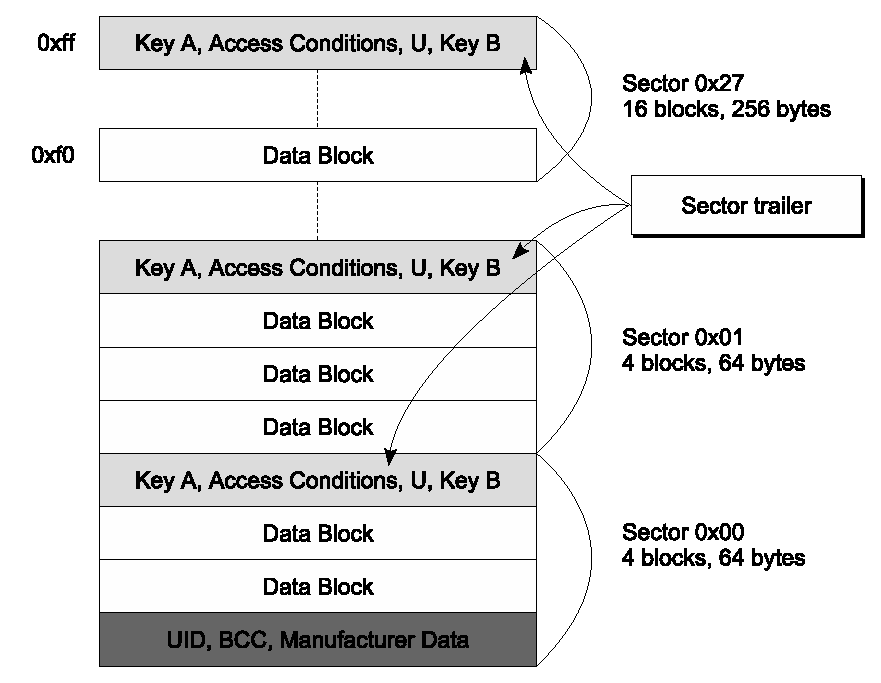
\includegraphics{figures/mifarememory1.eps}}
\caption{MIFARE Classic memory organisation}
\label{mifarememory1}
\end{figure}

The sector trailer itself has specific access conditions. Key A is never readable and key B can be configured to be readable or not. In the latter case, the sector is used just for data storage and only key A can be used to authenticate to the sector. Besides the keys and access conditions, there's one data byte (U) remaining, which has no defined purpose. A diagram of the sector trailer is shown in \autoref{mifarememory2}.

\begin{figure}[tbh]
\centerline{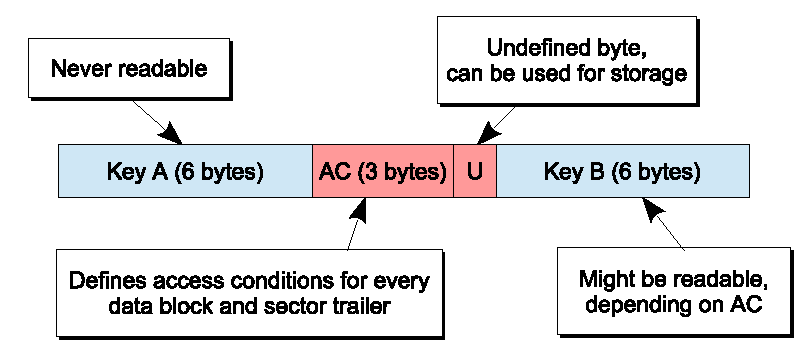
\includegraphics{figures/mifarememory2.eps}}
\caption{Sector trailer}
\label{mifarememory2}
\end{figure}

\subsection{Vulnerabilities}
\label{mifarevulnerabilities}

A number of weakness and vulnerabilities have been discovered in the MIFARE Classic system, including brute-forcible keys, a predictable pseudo-random number generator (PRNG), a cloning attack, and two very powerful attacks named the nested authentication attack and the Dark-Side attack. We shall discuss these vulnerabilities in the following paragraphs.

\subsubsection{Brute-forcing the sector keys}

As stated above, sector keys (A and B) are only 48 bits long, meaning they're vulnerable to a brute-force attack. This involves trying all $2^{48}$ possible keys one-by-one until the correct key is found. It has been shown that this can be done on dedicated hardware\footnote{FPGAs or GPUs.} in a matter of hours \cite{mifarebruteforce}.

\subsubsection{Predicting the output of the card's PRNG}

A PRNG is supposed to generate a sequence of numbers that are effectively indistinguishable from random or, put another way, an adversary should not be able to guess the next number in the sequence. In MIFARE Classic, the on-card PRNG plays an important role in the sector authentication protocol, CRYPTO-1. Specifically, it turns out that if we can predict the output of the PRNG, we're able to authenticate to sectors for which we do not know either of the keys -- this is the nested authentication attack, which is explained in the next paragraph. It was discovered that the output of the MIFARE Classic PRNG depends only on the amount of time that has elapsed since the card was powered up by the reader and that the PRNG has a period of 0.618 s. Thus, its output is entirely predictable, making the following attack possible.

\subsubsection{Nested authentication attack}

This attack allows an adversary to obtain all the keys for every sector on the card if just one key (A or B) is known for any sector. A readily available list of known default keys for MIFARE Classic cards exists and, unfortunately, many systems do not update these keys before issuing cards. When testing my own University of Cambridge card, I discovered that five of the sector keys used by the card were default keys.

When a reader attempts to authenticate to a sector on a card, the card produces a nonce, generated by the weak on-card PRNG, which it sends to the reader. Both the card and reader then derive some key stream bits using this nonce and the key for the sector (one of A or B). The trick here is that, once the reader has authenticated to a sector, subsequent authentication requests are encrypted. Furthermore, upon receiving an authentication request for a new sector, the card sets the internal state of the cipher to the key for the new sector. Thus, when the card sends the \emph{encrypted} nonce for a subsequent authentication request, since we are able to predict the nonce value, we can discover the key stream bits -- the first 32 bits of the sector key -- used to encrypt it by XORing the encrypted nonce with our prediction. Now we can easily brute-force the last 16 bits of the key.

\subsubsection{Dark-Side attack}

This attack allows an adversary to recover any key for any sector without any prior knowledge of any keys. During the authentication protocol, there's a single step where the reader sends encrypted data to the card, along with 8 parity bits. Parity bits are used in communication as a method for error detection/correction. It was noticed that if random data was sent by the reader, then with probability $1/256$, the card will respond in an unexpected way. The reason for this is that if any parity bits are wrong, the card won't respond at all. However, if all the parity bits are correct, but the corresponding data sent by the reader is not correct\footnote{The details of what a ``correct'' response is are specific to the authentication protocol. See \cite{darkside} for more information.}, the card responds with a 4-bit error code, 0x5 (NACK), which is encrypted. Since the plaintext is known, the attacker can recover the four key stream bits used to encrypt the NACK. By repeating this procedure many times, the internal state of the cipher can be discovered, allowing the attacker to completely reconstruct the sector key.

\subsubsection{Combined attack}

The combination of the nested authentication and Dark-Side attacks allows an adversary to completely recover all the keys from any card. They can first run the nested attack to determine if any default keys are in use. If this is not the case, they instead run the Dark-Side attack to recover just one key for any sector. With this one key, they can then rerun the nested attack to recover all other keys.

\subsubsection{Cloning cards}

Once all the keys have been recovered from a card, all the data can be read from it and written to another card, producing a clone. There's one slight issue here, however. As mentioned earlier, the first block of the first sector of a MIFARE Classic card contains a special piece of \textbf{read-only} data -- the UID. On legitimate MIFARE Classic cards, this value is burned onto the card during manufacturing, and is indeed unchangeable. However, there exist unofficial cards which emulate the MIFARE Classic system and have a programmable UID.\footnote{Such as the Fundan Microelectronics FM11RF08.} With one of these cards, an adversary is able to create an exact clone of any legitimate card.

\chapter{Preparation}

\section{Starting point}

This project makes significant use of the material from Security I and Security II. Further, material from Object-Oriented Programming and Further Java was utilised when writing the smart card application that runs on the JavaCard platform, which supports a subset of the Java language.

A previous attempt was made at this project by Denys Natykan, and so his 2017 Part II dissertation deserves mention. However, there're rather significant differences in our end products, as I opted to implement a different authentication protocol in order to complete certain extensions.

\section{Communication between card and reader}

The format for communication between a card and a reader is defined by ISO 7816-4 \cite{ISO78164}. It states that the basic unit of communication is the application protocol data unit (APDU). There are two categories of APDUs: commands APDUs and response APDUs. The reader is always the party that initiates communications and thus only ever sends command APDUs. Correspondingly, the card always waits for commands from the reader and thus only ever sends response APDUs.

\subsection{Command APDU}

Command APDUs consist of a required 4-byte header and an optional body. The header contains the following four elements, each 1-byte long:

\begin{itemize}
\item CLA -- indicates the class of command, interindustry or proprietary.
\item INS -- instruction code, indicates the specific command, e.g. ``initiate authentication''.
\item P1, P2 -- instruction parameters, these are command specific.
\end{itemize}

\noindent
The optional body contains the following three elements:

\begin{itemize}
\item L\textsubscript{c} -- either 0, 1 or 3 bytes encoding the number (N\textsubscript{c}) of bytes of command data to follow.
	\begin{itemize}
	\item If the L\textsubscript{c} field is absent, then N\textsubscript{c} is zero.
	\item A short L\textsubscript{c} field consists of one byte not set to \texttt{0x00}, allowing a value of N\textsubscript{c} up to 255.
	\item An extended L\textsubscript{c} field consists of three bytes: one byte set to \texttt{0x00} followed by two bytes not set to \texttt{0x0000}, allowing a value of N\textsubscript{c} up to 65,535.
	\end{itemize}
\item Command data -- N\textsubscript{c} bytes of data.
\item L\textsubscript{e} -- between 0--3 bytes encoding the maximum number (N\textsubscript{e}) of response bytes expected.
	\begin{itemize}
	\item If the L\textsubscript{e} field is absent, then N\textsubscript{e} is zero.
	\item A short L\textsubscript{e} field consists of one byte with any value -- if the byte is set to \texttt{0x00}, then N\textsubscript{e} is 256.
	\item An extended L\textsubscript{e} field consists of either three bytes (one byte set to \texttt{0x00} followed by two bytes with any value) if the L\textsubscript{c} field is absent, or two bytes with any value if an extended L\textsubscript{c} field is present, where the value \texttt{0x0000} corresponds to N\textsubscript{e} equal to 65,536.
	\end{itemize}
\end{itemize}

\noindent
If the body is included, parts can be left out depending on the requirements, e.g. if the command has no data, but a response is expected, only the L\textsubscript{e} field will be present. Similarly, if the command has data but doesn't expect a response, only the L\textsubscript{c} and command data fields will be present. A diagram of the structure of a command APDU is shown in \autoref{commandapdu}.

\begin{figure}[tbh]
\centerline{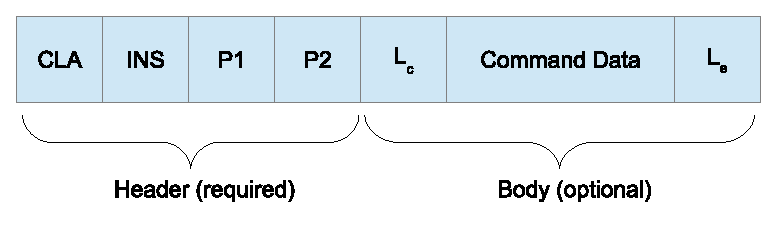
\includegraphics{figures/commandapdu.eps}}
\caption{Command APDU}
\label{commandapdu}
\end{figure}

\subsection{Response APDU}

Response APDUs consist of an optional body and a required 2-byte trailer. The optional body contains any response data the card wishes to send to the reader, and should not exceed N\textsubscript{e} bytes in length. The trailer contains two \emph{status word} bytes, SW1 and SW2, which indicate the command processing status (e.g. 0x9000 indicates no error, command success, whereas 0x6A80 indicates wrong data). A diagram of the structure of a response APDU is shown in \autoref{responseapdu}.

\begin{figure}[tbh]
\centerline{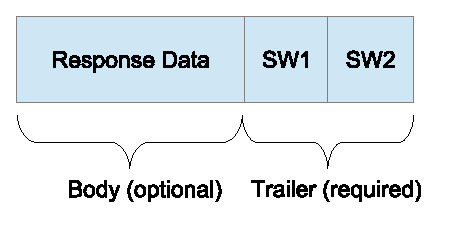
\includegraphics{figures/responseapdu.eps}}
\caption{Response APDU}
\label{responseapdu}
\end{figure}

\section{JavaCard}

The JavaCard platform allows Java-based applets to be run securely on smartcards with limited memory and processing capabilities. The choice to use a smartcard that implemented JavaCard was made for a few reasons. Firstly, the development ecosystem is very mature -- Sun (and later Oracle) make available extensive documentation and resources, perhaps most importantly of which are detailed API references. One article in particular was an excellent introduction to writing JavaCard applets \cite{writingapplets}. There's also an active development community, and I was able to find solutions to many of the problems that arose during the implementation stage by searching forums.\footnote{E.g. https://www.javacardos.com/javacardforum and Stack Overflow.} Because of the fact that JavaCard uses a subset of the Java language, there's no chance for security vulnerabilities resulting from pointer arithmetic. JavaCard also makes extending a card's functionality very simple, as multiple applets can be deployed on a card and new applets can be installed even after a card has been issued.

\subsection{Language}

The JavaCard Virtual Machine (JCVM) specification defines an allowed subset of the Java programming language. Perhaps one of the biggest differences is that only the \texttt{boolean}, \texttt{byte} and \texttt{short} types are permitted -- support for \texttt{int} is optional, and the card I used for this project didn't support it. Further, JavaCard does not require a garbage collector and so one may not assume that objects which are allocated are ever deallocated. A further discussion of memory occurs in \autoref{javacardmemory}. Multi-threading is not supported; although multiple applets can reside on a card, only one can be active at any one time.

\subsection{JavaCard Virtual Machine}

The VM for the JavaCard platform is implemented in two parts, with one part external to the card and the other running on the card itself. The on-card VM interprets bytecode, manages classes and objects, and so on. The external part, referred to as the \emph{converter tool}, loads, verifies, and further prepares the Java classes in a card applet for on-card execution. The output of the converter tool is a Converted Applet (CAP) file, a file that contains all the classes in a Java package in a loadable, executable binary representation. The converter verifies that the classes conform to the Java Card specification. The CAP file can then be installed onto a card.

\begin{figure}[tbh]
\centerline{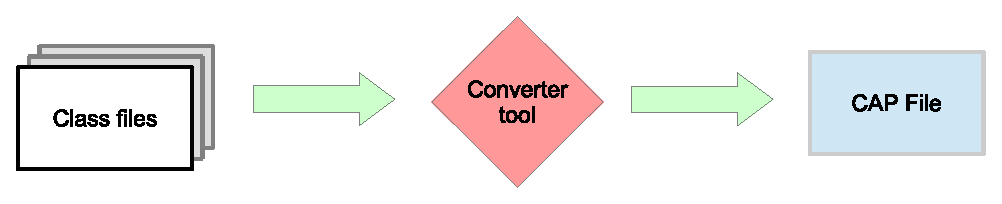
\includegraphics{figures/capconverter.eps}}
\caption{CAP Converter Tool}
\label{capconverter}
\end{figure}

\subsection{Applets}
\label{sec:applets}

Applications that run on the card are called applets. Each applet on the card must be uniquely identified by an Application ID (AID). An AID, as defined in ISO 7816-5 \cite{ISO78165}, is a sequence of between 5 and 15 bytes. All applets must extend the \texttt{javacard.framework.Applet} abstract base class.

\subsubsection{Applet life-cycle}

The applet life-cycle begins when the applet is downloaded to the card and the JavaCard Runtime Environment (JCRE) invokes the applet's static \texttt{Applet.install()} method, and the applet registers itself with the JCRE by invoking \texttt{Applet.register()}. Once the applet is installed and registered, it is in the unselected state, available for selection and APDU processing. While in the unselected state, the applet is inactive. An applet gets selected for APDU processing when the host application asks the JCRE to select a specific applet in the card (by instructing the card reader to send a \texttt{SELECT} APDU). To notify the applet that a host application has selected it, the JCRE calls its \texttt{select()} method; the applet typically performs appropriate initialization in preparation for APDU processing.

Once selection is done, the JCRE passes incoming APDU commands to the applet for processing by invoking its \texttt{process()} method.

Applet deselection occurs when the host application tells the JCRE to select another applet. The JCRE notifies the active applet that it has been deselected by calling its \texttt{deselect()} method, which typically performs any clean-up logic and returns the applet to the inactive, unselected state. If power is lost, the applet is reset to the inactive state without the \texttt{deselect()} method being called. \autoref{appletlifecycle} summarises the applet life-cycle.

\begin{figure}[tbh]
\centerline{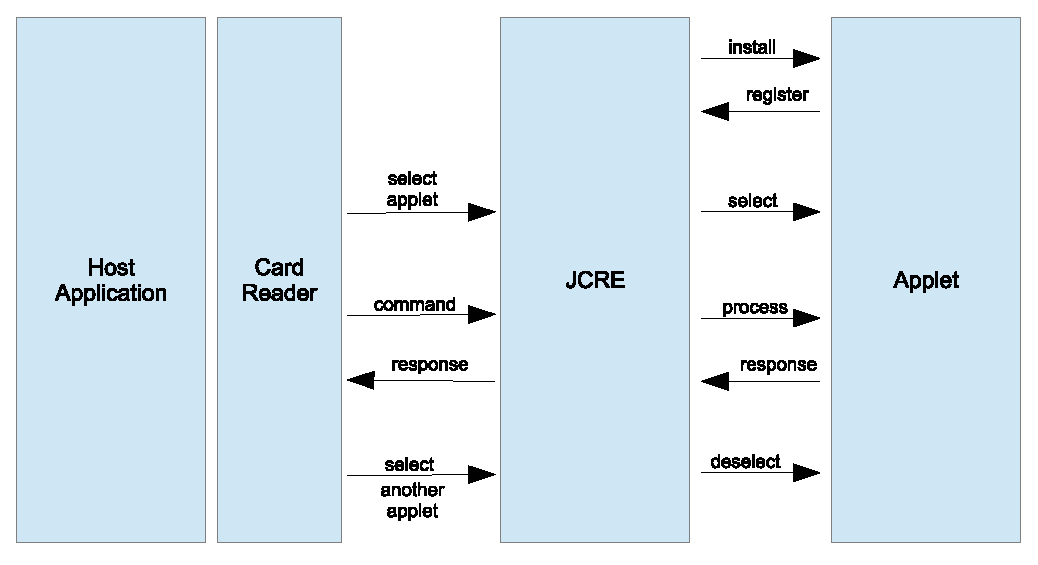
\includegraphics{figures/appletlifecycle.eps}}
\caption{Applet Life-Cycle}
\label{appletlifecycle}
\end{figure}

\subsection{Memory organisation} \label{javacardmemory}

JavaCard smartcards offer two types of memory: transient Random Access Memory (RAM) and persistent Electronically Erasable Programmable Read-Only Memory (EEPROM). Typically, much more EEPROM than RAM is available -- the NXP J3A040 has 40KB of EEPROM but roughly 6KB of RAM. However, RAM read/write speeds are faster by an approximate factor of $10^3$.

\subsubsection{Transient RAM}

Transient memory is erased on power down and is thus only suitable for storing temporary data. As an example, during execution of the OPACITY-FS inspired protocol described in this dissertation, several encryption keys must be derived using a key derivation function (KDF). These keys are only needed for the duration of the protocol execution, and thus do not need to persist when the card loses power. Therefore, it would be perfectly suitable to use transient buffers to hold them.

Transient objects can only be created via the JavaCard API, e.g. to create a transient byte array, one must call \texttt{JCSystem.makeTransientByteArray()}. Note that, although the actual memory is transient, the reference that points to the memory is persistent. Thus a transient object should only ever be created once, and the ideal place to do this is in the applet's constructor (which should be called by the \texttt{install()} method).

\subsubsection{Persistent EEPROM}

Anytime the \texttt{new} keyword is used, a persistent object will be created. Further, all of a class' instance variables and static variables, as well as local variables within its methods, will be stored in persistent memory. As stated earlier, certain cards do not actually have a garbage collector. Thus it's very important to ensure careful use of EEPROM, since once created, an object may never be erased and memory leaks can easily occur. Writes to EEPROM are atomic, meaning that there's no need for concern over data inconsistencies in the event that power is unexpectedly lost, e.g. because the card is moved out of the range of the reader. Unfortunately, writes also wear out the physical memory circuit, and thus frequent writes will reduce the lifetime of the card. In order to mitigate this effect, I was careful to ensure that any data that could be, was stored in RAM.

\section{Resources}

\subsection{Physical resources}

Before I was able to begin the implementation stage, I ordered the following items:

\begin{itemize}
\item Identiv SCL3711 -- A USB smartcard reader. I had originally intended to use this reader, but discovered that, despite the claims of the manufacturer, it was not compatible with my operating system (OSX 10.11, El Capitan).
\item ACS ACR122T -- alternative USB smartcard reader that was compatible.
\item NXP J3A040 CL -- a programmable contactless-only smartcard with 40K of EEPROM memory, implementing JavaCard 2.2.2 and Global Platform 2.1.1, and conforming to ISO 14443-A. I chose this card because it is relatively cheap and it supports many of the cryptographic algorithms that I needed in order to implement an authentication protocol based on asymmetric cryptography\footnote{E.g. support for ECDSA (and AES, which is used in the mutual authentication protocol that I implemented).}. Note that cards may support some algorithms but only for certain key sizes. For example, the J3A040 only supports ECDSA keys of up to 192 bits. Details of what algorithms and key sizes a card supports can be found by using JCAlgTest \cite{jcalgtest}.
\end{itemize}

\subsection{GlobalPlatform and GPShell}

The GlobalPlatform card specification is a standard for the management of the infrastructure of a smartcard, the most relevant tasks being installation and removal of applications on a card. GPShell \cite{gpshell} is a script interpreter used for talking to smartcards that are compliant with the GlobalPlatform card specification. It can establish a secure channel with a smartcard in order to load, instantiate, delete and list applications on the card. \autoref{gpinstall} shows the script I use to install a CAP file called \texttt{opacity\_fs\_impl.cap} onto a card. The script commands are converted, by GPShell, to command APDUs which are sent to the card via the connected reader.

\begin{lstlisting}[caption={Applet install script},captionpos=b,label={gpinstall}]
enable_trace
establish_context
mode_211
card_connect
select -AID a0000000030000
open_sc -security 1 -keyind 0 -keyver 0
    -mac_key 404142434445464748494a4b4c4d4e4f
    -enc_key 404142434445464748494a4b4c4d4e4f
delete -AID f234123456101000
install -file opacity_fs_impl.cap -sdAID a000000003000000 -priv 2
    -nvDataLimit 5000
card_disconnect
release_context
\end{lstlisting}

\begin{itemize}
\item \texttt{enable\_trace} -- writes a log of all command/response APDUs (hex encoded) to standard output.
\item \texttt{establish\_context} -- before any communication can by done to any card this command must be executed.
\item \texttt{mode\_211} -- sets the protocol mode to GlobalPlatform 2.1.1.
\item \texttt{card\_connect} -- connect to card via reader.
\item \texttt{select -AID a0000000030000} -- select the \emph{card manager} applet. The card manager understands command APDUs for installing/deleting applets. The AID of the card manager is card-specific and may be found in the datasheet.
\item \texttt{open\_sc -security 1 -keyind 0 -keyver 0 -mac\_key 404142434445464748494a4b4c4d4e4f -enc\_key 404142434445464748494a4b4c4d4e4f} -- open a secure channel to the card with the standard JavaCard Open Platform (JCOP) keys; the J3A040 CL is a JCOP card.
\item \texttt{delete -AID f234123456101000} -- delete the applet with the given AID. This was the AID I used for my applet, so this step is just to remove any old version of the applet before installing the new one.
\item \texttt{install -file opacity\_fs\_impl.cap -sdAID a000000003000000 -priv 2 -nvDataLimit 5000} -- install the file named \texttt{opacity\_fs\_impl.cap} and limit its non-volatile (EEPROM) data allowance to 5KB. An option specifies the \emph{security domain} AID (sdAID), which in this case is the card manager.
\item \texttt{card\_disconnect} -- disconnect the card.
\item \texttt{release\_context} -- release the context that was established at the beginning of the script.
\end{itemize}

\subsection{Build tools}

I used Apache Ant \cite{ant} to build all my applications. In combination with a useful Ant task\footnote{https://github.com/martinpaljak/ant-javacard}, I was able to build and convert the card application to a CAP file in one command. The build file I used for the card application can be found in \autoref{appendix:cardappbuildfile}.

\subsection{Source control}

I used Git for source control, regularly pushing to a remote Bitbucket repository. This allowed me to save the state of the project as various development milestones were achieved.

\subsection{External libraries}

Four external libraries were used in this project. The first of these was the Apache Commons Codec \cite{apachecommonscodec} library, which was useful because of the \texttt{org.apache.commons.codec.binary.Hex} class, specifically the \texttt{encodeHexString()} method. This allowed me to analyse the card's responses in a readable format and was helpful for debugging. The second was the Bouncy Castle \cite{bouncycastle} library, which I used as a provider. In Java, a ``provider'' implements the Java security API, for instance by providing implementations of cryptographic algorithms (ECDSA, SHA-1) or classes for key generation and management. As well as acting as a provider, it offered a handful of useful methods that the standard Java API didn't, for example a method for obtaining a byte array of the encoding of a public ECDSA key. The third was the Apache Commons CLI \cite{apachecommonscli} library, which was helpful in parsing flags and arguments passed to the provisioning application. The final library was the JavaCard 2.2.2 SDK.

\section{Development strategy}

I chose to adopt an agile development strategy for the implementation phase of the project. The core principle behind agile development is that working software is the primary measure of progress. Thus, at the outset, I broke the project down into small parts that could each be designed, implemented and tested within a very short timeframe, perhaps one or two weeks. This strategy of development allowed me to adapt to issues inherent in my original plan (which could not have been forseen) with relative ease.

\chapter{Implementation}

The project consists of three applications: the card-provisioning application, described in \autoref{provisionapp}, and two separate applications that implement the authentication protocol, one that runs on the card, the other on the reader. Two authentication protocols were devised for the project -- the first protocol, described in \autoref{basicauth}, is very basic and only authenticates the card's identity. The second, described in \autoref{mutualauth}, performs mutual authentication and provides strong privacy properties.

\section{Card-provisioning application}
\label{provisionapp}

Both authentication protocols are built around elliptic curve (EC) cryptography, and thus it was necessary to write a command-line application that provisions cards with a signed EC key pair. The application is also able to generate a key pair that it will use for signing card key pairs, and lastly, there's a command for signing a provided file (the reason for this is explained below). \autoref{provisionhelp} shows the help output of the application.

\begin{figure}[tbh]
\centerline{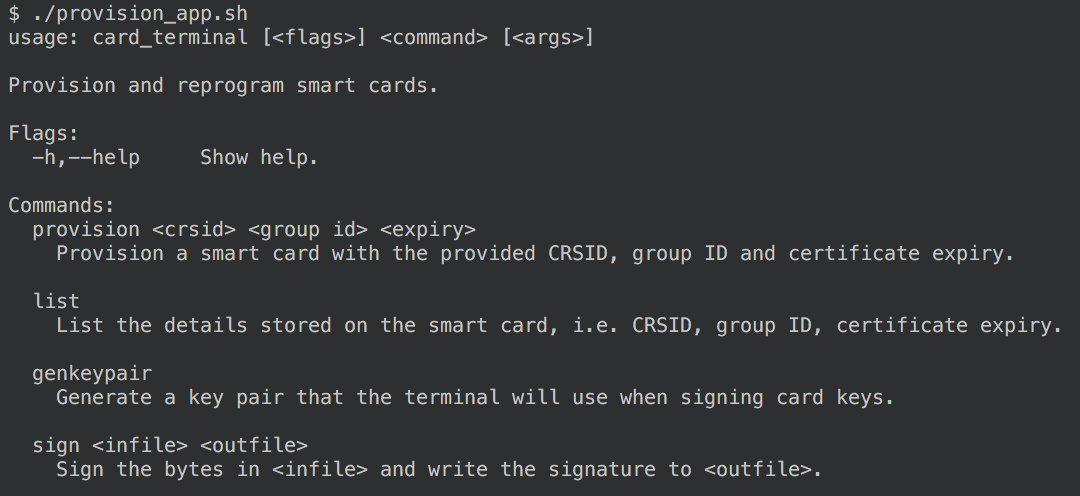
\includegraphics[scale=0.7]{figures/provisionhelp.png}}
\caption{Card-provisioning application help output}
\label{provisionhelp}
\end{figure}

Note that the provision command takes as input three items: CRSID, a \emph{group ID}, and a card expiry date. These items, along with the card's public key, are all included as part of the input data when generating the card's ECDSA signature.

\subsubsection{Card-provisioning terminal key pair}

In order to generate ECDSA signatures, the card terminal needs a key pair of its own. This can be generated using the \texttt{genkeypair} command. It's important that this key pair is kept safe, since all cards and readers contain a copy, in order to perform the mutual authentication protocol. Thus, if it has to be replaced (e.g. if it was accidentally deleted or overwritten), then all cards and readers will have to be re-provisioned. Further, if it falls into the hands of an adversary, then they could provision cards with whatever access permissions they choose.

\subsubsection{Provisioning readers}

In order to perform mutual authentication, readers must also have their own signed EC key pair. The \texttt{sign} command exists for this reason. Once a reader has generated its key pair, the \texttt{sign} command can be called, with the \texttt{<infile>} argument being the reader's public key. Readers also need a copy of the provisioning terminal's public key in order to be able to authenticate card signatures. Both the signature and terminal public key can then be loaded when the reader-side authentication application starts.

\subsection{Format of CRSID}

The CRSID is stored on the card in a byte array. When the provisioning application retrieves the CRSID from the command-line arguments, it converts it to a byte array using the \texttt{getBytes()} method from Java's \texttt{String} class. This method encodes the CRSID using a character set, which is provided as an argument. For this project, the chosen character set was UTF-8, thus CRSIDs may only contain UTF-8 characters.

\subsection{Format of group ID}

The group ID specifies the access permissions of the card. It is variable-length, and thus no format has been hard-coded into the implementation. One possible option is to have each bit correspond to a certain location. If the bit is set, then the card has access to that location. For example, the sixth bit being set could correspond to permission to access a certain faculty. This format would make the group ID easily extensible.

\subsection{Format of card expiry date}

The card expiry date is stored as a 4-byte array, representing a 32-bit \emph{unsigned} integer. This integer corresponds to the number of seconds between the expiry date and 01/01/1970 00:00:00 (UTC). This is similar to Unix time, except for the fact that Unix time is stored as a \emph{signed} 32-bit integer.

\subsection{Card provisioning protocol}

The provisioning protocol is very straightforward. First, the provisioning terminal sends a command APDU to the card telling it to generate an ECDSA key pair. The card replies with a response APDU containing its public key, encoded according to SEC1 \cite{sec1} \S2.3.3. The reader then produces an ECDSA signature, using as input the following items concatenated together in a byte array: CRSID, group ID, card expiry date and card public key. It then sends a \texttt{STORE} command to the card, with the signature, CRSID, group ID, card expiry and its own public key\footnote{As mentioned earlier, the terminal's public key is needed in order for the card to be able to verify a reader's identity during the mutual authentication protocol.} in the body of the APDU. The card copies these items to persistent memory and responds with a ``command success'' status word (0x9000). The reader then sends a \texttt{CHECK} command, where the card returns all the data that it just stored -- this step is to ensure no data corruption occurred. If all the data is correct, the reader sends a final \texttt{LOCK} command, after which the card will not respond to any of the earlier commands until unlocked. A diagram of the provisioning protocol is shown in \autoref{provisioningprotocol}.

\begin{figure}[tbh]
\centerline{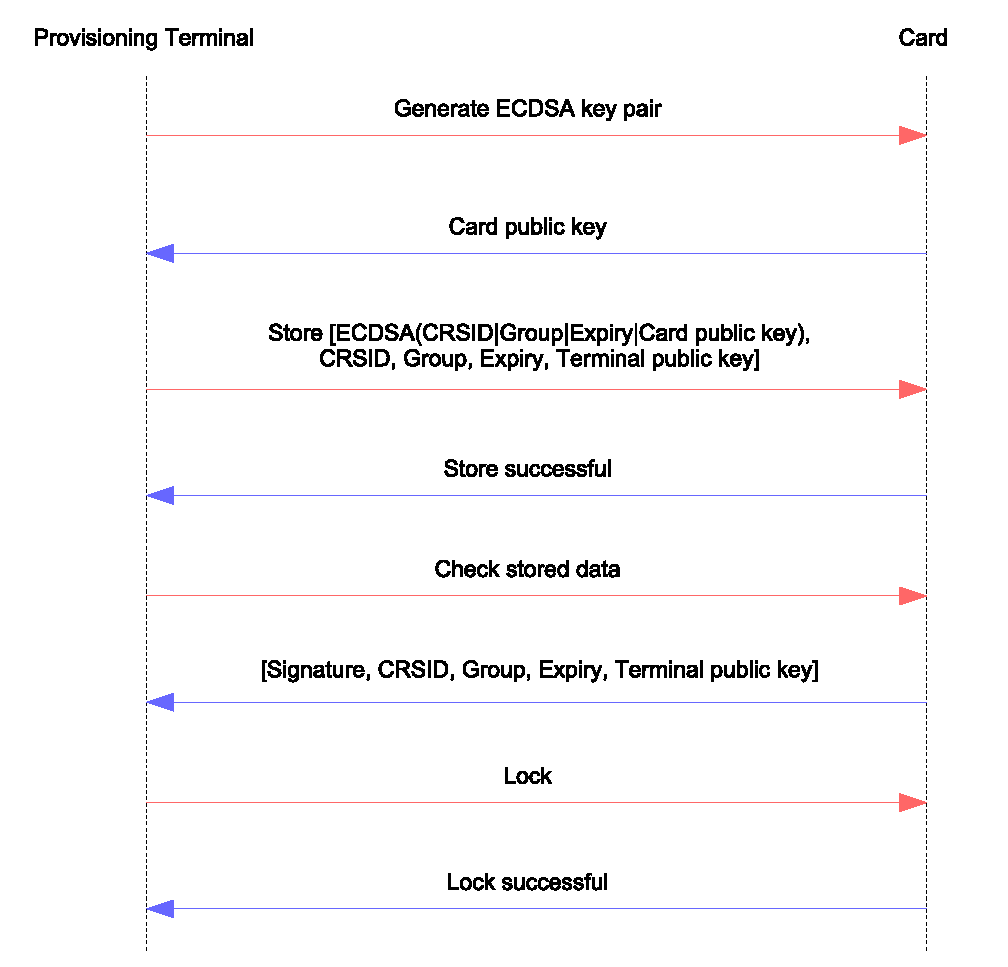
\includegraphics[scale=0.8]{figures/provisioningprotocol.eps}}
\caption{Card-provisioning protocol}
\label{provisioningprotocol}
\end{figure}

\subsubsection{ECDSA signature format}

Distinguished Encoding Rules (DER) is the data format used to encode an ECDSA signature, which is defined by SEC1 as an Abstract Syntax Notation One (ASN.1) sequence of two integers \texttt{r} and \texttt{s}.

\begin{lstlisting}[caption={ASN.1 structure of an ECDSA signature},captionpos=b]
ECDSASignature ::= SEQUENCE {
    r    INTEGER,
    s    INTEGER
}
\end{lstlisting}

\noindent
The following sequence of bytes shows the DER encoding of an ECDSA signature: \texttt{0x30 b1 0x02 b2 (vr) 0x02 b3 (vs)}.

\begin{itemize}
\item \texttt{0x30} signifies the start of a sequence.
\item \texttt{0x02} signifies the start of an integer.
\item \texttt{b1} is a single byte value, equal to the length, in bytes, of the remaining sequence of bytes (from the first \texttt{0x02} to the end of the encoding).
\item \texttt{b2} is a single byte value, equal to the length, in bytes, of \texttt{(vr)}.
\item \texttt{b3} is a single byte value, equal to the length, in bytes, of \texttt{(vs)}.
\item \texttt{(vr)} is the signed, big-endian, minimal length encoding of the value \texttt{r}.
\item \texttt{(vs)} is the signed, big-endian, minimal length encoding of the value \texttt{s}.
\end{itemize}

\noindent
\emph{Minimal length} means that the total length is the shortest possible to represent the value, and \emph{signed} means that the first bit of the first byte specifies the sign of the value. Since \texttt{r} and \texttt{s} are always positive, the first bit of the first byte of both \texttt{(vr)} and \texttt{(vs)} must be \texttt{0}, i.e. the first byte must have a value between \texttt{0x00} and \texttt{0x7F}. If the minimal, \emph{unsigned} representation of either value has a first byte with value greater than \texttt{0x7F}, the DER-encoded representation must be padded with an \texttt{0x00} byte.

The relevance of this is that JavaCard and Bouncy Castle treat signatures slightly differently. JavaCard does not adhere to the ``minimal length'' criteria and always pads \texttt{(vr)} and \texttt{(vs)} with zeros until the signature is the maximum allowed length -- in fact, JavaCard will not be able to decode a signature \emph{unless} it has maximal length. Thus, before sending a signature generated by Bouncy Castle to a card, it must be padded to the maximum length. Equally, when we receive a signature generated by JavaCard, we must remove any incorrectly inserted pads (zeros), else Bouncy Castle will not be able to decode it. This particular issue was extremely difficult to debug.

\section{Basic authentication protocol}
\label{basicauth}

The basic authentication protocol is relatively simple. The reader begins by generating a 100-byte cryptographic nonce.\footnote{A nonce is a random number, normally used for the purpose of preventing a replay attack.} The reader sends this nonce to the card in the body of a \texttt{BASIC\_AUTH} command. The card generates an ECDSA signature, using the nonce as the input data. It then returns this nonce signature, along with its stored CRSID, group ID, expiry date, EC public key and card signature\footnote{This was the signature stored during provisioning.}, in the body of a response APDU. The reader first verifies the card signature to ensure the card's public key is valid, then checks the card expiry date. Having done that, it verifies the nonce signature to ensure that the card it's communicating with has the matching private key\footnote{Otherwise it's possible that an attacker could just be replaying an old communication; the nonce signature prevents this possibility.}. Finally, the reader checks that the group ID permits access to the location in question. A diagram of the protocol is shown in \autoref{fig:basicauth}.

\begin{figure}[tbh]
\centerline{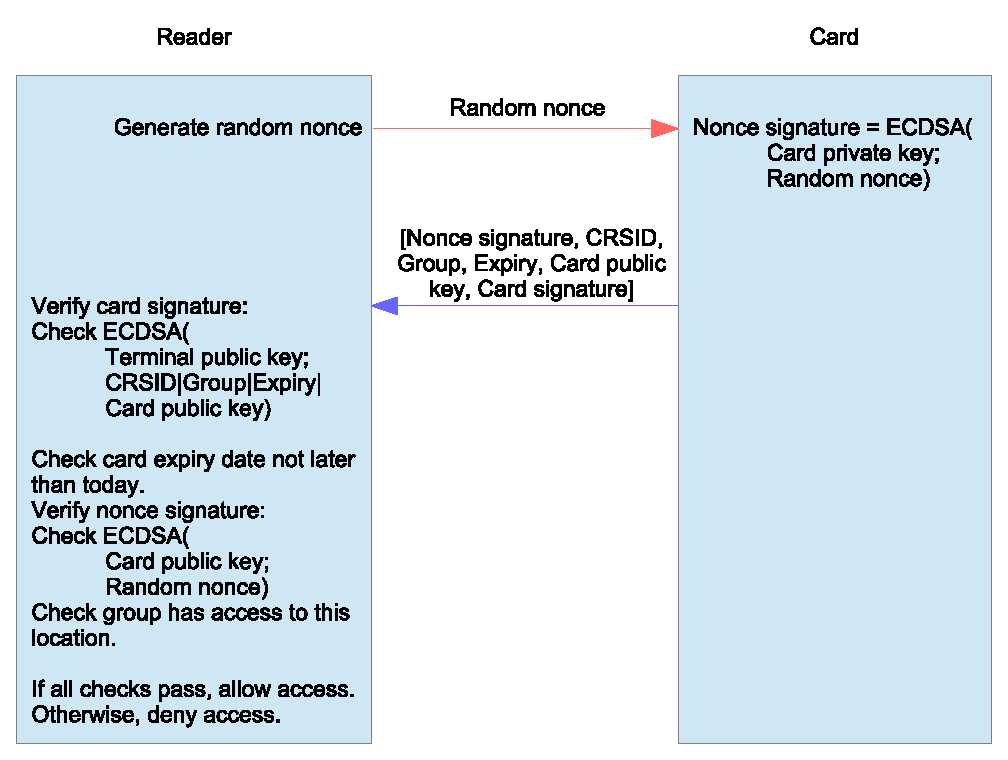
\includegraphics[scale=0.8]{figures/basicauth.eps}}
\caption{Basic authentication protocol}
\label{fig:basicauth}
\end{figure}

\section{Mutual authentication protocol}
\label{mutualauth}

The mutual authentication protocol is based on the OPACITY \cite{OPACITY} Full Secrecy (FS) protocol, the main difference being the omission of persistent binding. The reason for this is explained in \autoref{opacityomissions}.

This protocol is quite different from the basic protocol, in that it uses EC Diffie-Hellman (ECDH) as the main asymmetric key algorithm, instead of ECDSA. Further, ephemeral EC key pairs play the role of nonces -- that is, to protect against replay attacks. Regarding notation, $d_{xy}$ refers to a private EC key, where $x$ is either $e$, meaning ephemeral, or $s$, meaning permanent\footnote{The permanent keys are the ones given to the reader and card during provisioning.}, and $y$ is either $H$, the reader (host), or $ICC$, the card (integrated circuit card). For example, $d_{eICC}$ refers to the card's ephemeral private key. In a similar way, $Q_{xy}$ refers to a public key. $C_{H}$ refers to the reader's \emph{certificate}, which is simply its permanent public key and the matching signature. $C_{ICC}$ refers to the card's certificate, which includes all the data used to generate the card signature, as well as the signature itself. $T_x(y)$ means the top (most significant) $x$ bits of $y$. Finally, $SK$ refers to a symmetric key.

The protocol begins with the reader generating an ephemeral key pair, ($d_{eH}$; $Q_{eH}$). The reader then sends the card its certificate, $C_H$, and the public ephemeral key, $Q_{eH}$. The card validates $C_H$ using the provisioning terminal's public key, which it stored during provisioning, and extracts $Q_{sH}$. Before proceeding, it ensures that $Q_{eH}$ is a valid EC key.\footnote{Further, it checks that the key belongs to the EC domain. For this project, the Prime192v1 curve was used.} It then generates its own ephemeral key pair, ($d_{eICC}$; $Q_{eICC}$). Now, it derives a secret, $Z1$, by performing ECDH with ($d_{eICC}$; $Q_{sH}$). By passing this secret to a key derivation function (KDF), it derives two secret keys, $K1$ and $K2$. The card encrypts its own certificate, $C_{ICC}$, using AES-128 with $K1$, to get $OpaqueData_{ICC}$. A second secret, $Z$, is derived using ECDH with ($d_{sICC}$; $Q_{eH}$). Now a third secret key, $SK_{CFRM}$ is derived by passing $Z$ to a KDF. $K2$ is also used by the KDF in deriving $SK_{CFRM}$. The final card-side step is to generate a message authentication code (MAC). The card generates this MAC using CBC-MAC, with AES-128 as the underlying block cipher and $SK_{CFRM}$ as the key. The data passed to CBC-MAC is $T_8(Q_{eICC})$ concatenated with $T_{16}(Q_{eH})$. The MAC is referred to as $AuthCryptogram_{ICC}$. Once all this has been done, the card responds to the reader with ($OpaqueData_{ICC} \vert AuthCryptogram_{ICC} \vert Q_{eICC}$). The reader then essentially mirrors this exact sequence of computations with two key differences. Firstly, the ECDH calls use different keys, since private keys may never leave their owner. For example, to derive $Z1$, the reader calls ECDH with ($d_{sH}$; $Q_{eICC}$) instead of ($d_{eICC}$; $Q_{sH}$). Notice that because we used $d_{eICC}$ on the card-side, we use $Q_{eICC}$ on the reader-side, and similarly for the other two keys used. The nature of ECDH is that if this is the case, the derived secret is the same for both calls. Thus the two sides can derive the same secret without revealing their private keys. The other difference is that instead of encrypting the card certificate, the reader will decrypt $OpaqueData_{ICC}$ to \emph{retrieve} $C_{ICC}$. Also, after checking that $AuthCryptogram_{ICC}$ matches the MAC that the reader produced, the reader will check the card's expiry date and group ID to ensure access is allowed. If all these checks pass, the reader grants access. A diagram of the protocol is shown in \autoref{fig:mutualauth}.

\begin{figure}[tbh]
\centerline{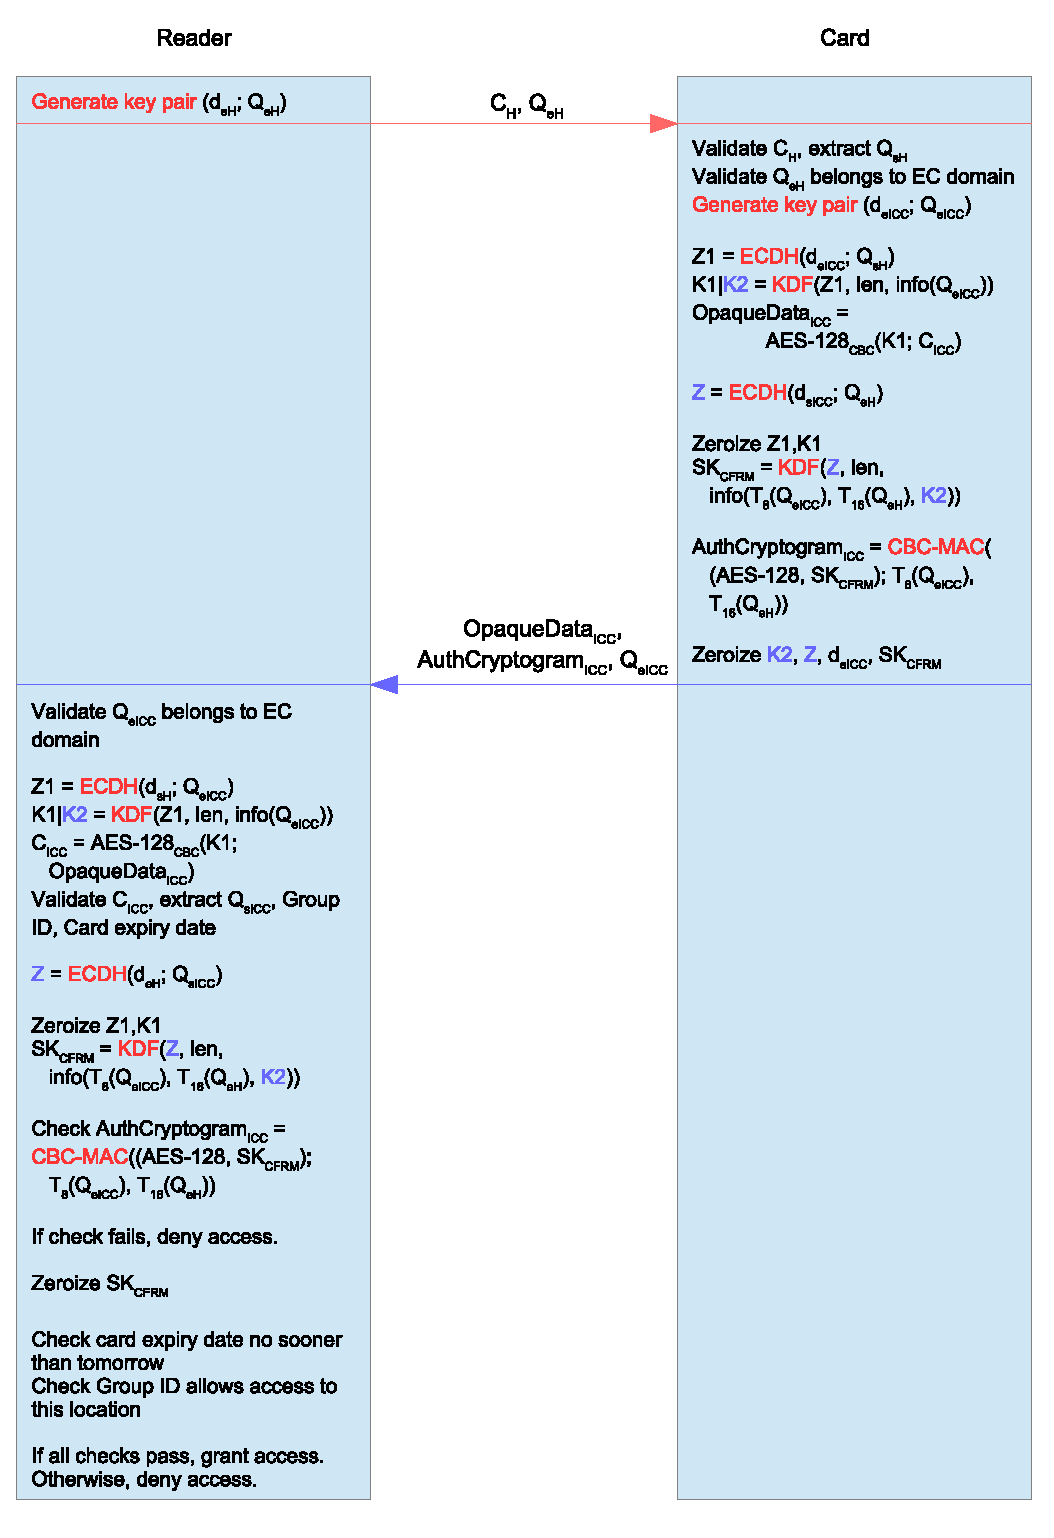
\includegraphics[scale=0.8]{figures/mutualauth.eps}}
\caption{Mutual authentication protocol}
\label{fig:mutualauth}
\end{figure}

\subsection{Concatenation KDF}

The KDF used in the protocol is the concatenation KDF as specified in NIST SP800-56A \cite{nistsp80056a} (\S5.8.1). JavaCard 2.2.2 does not support this KDF, and thus I had to implement it myself. It takes as arguments a key, the desired length of the derived keying material and some ``other information''. In the case of this protocol, the other information is defined as in Annex A of \cite{OPACITY}. Briefly, if $SK_1, ..., SK_p =  KDF(Z, keydatalen, info(A_1, ..., A_m)$, then $info(A_1, ..., A_m) = AlgoID(SK_1)~\vert~...~\vert~AlgoID(SK_p)~\vert~A_1~\vert~...~\vert~A_m$, where AlgoID for this protocol is always 0x09, the algorithm ID for an AES-128 key, as defined in Annex A of \cite{OPACITY}.

The concatenation KDF is built on an \emph{approved} hash function -- a list of such functions is given in FIPS 180-2 \cite{fips1802}. The algorithm is shown below:

\begin{center}
\begin{algorithm}[H]
\SetAlgoLined
\tcp{Compute the number of times the hash function must be called.}
\tcp{$hashlen$ is the length of the output of the chosen hash function.}
$reps \leftarrow \lceil \frac{keydatalen}{hashen} \rceil$\;
\tcp{Initialize a 32-bit, big-endian bit string to act as a counter.}
$counter \leftarrow 00000001_{16}$\;
\For{$i \leftarrow 1$ \KwTo $reps$}{
	\tcp{$H$ is the chosen hash function.}
	$Hash_i \leftarrow H(counter \vert Z \vert info(...))$\;
	$counter \leftarrow counter+1~(\bmod~2^{32}$)\;
}
\uIf{$keydatalen/hashlen$ is an integer}{$Hhash \leftarrow Hash_{reps}$\;}
\Else{$Hhash \leftarrow$ ($keydatalen~\bmod~hashlen$) leftmost bits of $Hash_{reps}$\;}
$DerivedKeyingMaterial \leftarrow Hash_1 \vert Hash_2 \vert ... \vert Hash_{reps-1} \vert Hhash$\;
\end{algorithm}
\end{center}

\noindent
Listing \autoref{concatkdf} shows the JavaCard implementation of the concatenation KDF loop.

\begin{listing}
\begin{minted}[linenos]{java}
for (short counter = (short)1; counter <= numBlocksToGenerate; counter++) {
  // Change the counter value in the hash input.
  Util.setShort(hashData, (short)(COUNTER_LENGTH-2), counter);
  hash.reset();
  // Compute the hash of hashData, and write the result to derivedKey,
  // a byte array that holds the derived keying material.
  hash.doFinal(hashData, (short)0, (short)hashData.length, derivedKey, offset);
  offset += KDF_HASH_OUTPUT_SIZE;
}
\end{minted}
\caption{The main loop of the concatenation KDF}
\label{concatkdf}
\end{listing}

\noindent
The concatenation KDF was implemented separately for the reader application. A number of test input vectors were fed to both KDF implementations and the results compared, to ensure the two implementations produced the same outputs.

\subsection{Mutual authentication}
\label{sec:mutualauth}

The basic authentication protocol described in \autoref{basicauth} only authenticates the card, i.e. the card cannot tell whether the reader is real (e.g. a reader controlling access to a university door) or adversarial (e.g. someone holding a USB reader up to a victim's pocket). Under such a protocol, the card may reveal sensitive information to an attacker. Even seemingly trivial data, such as a public key, can be used to track a card, and thus should not be divulged at will. The mutual authentication protocol solves this by doing the obvious thing -- authenticating both the card \emph{and} the reader. Strictly speaking, the protocol doesn't actually authenticate the reader. However, it works such that only a valid reader will be able to access sensitive information, which is the intention of mutual authentication, and so the distinction is semantic. This is achieved in a clever way. Notice that, in order to get any sensitive data from the card, the reader must be able to decrypt $OpaqueData_{ICC}$. Thus, it must be able to derive $K1$, which in turn means being able to derive $Z1$. Before continuing, recognise that an attacker could eavesdrop an exchange between a valid reader and card, and thus could know a valid certificate, $C_{H}$, and ephemeral public key, $Q_{eH}$. By replaying this information, the attacker could force a card to engage in the protocol. However, once the card responds with $OpaqueData_{ICC}$, since the attacker doesn't know $d_{sH}$, they cannot derive $Z1$, and therefore, ultimately, cannot decrypt the sensitive data. Notice also that an attacker cannot simply choose $C_{H}$ at random, since $Q_{sH}$ must be signed by the provisioning terminal. In this way, only valid readers are able to read a card's sensitive data.

\subsection{Privacy properties}

The mutual authentication protocol has strong privacy properties. In particular, it provides deniability, identity hiding and untraceability.

\subsubsection{Deniability}

Deniability is the inability to use transcripts of communications as proofs towards third parties, i.e. an outsider cannot prove that a specific card has communicated with a specific reader based on, for instance, transcripts of communications taken from logs stored by the reader. The protocol ensures a very basic level of deniability, protecting only against abuse of transcripts between a real card and reader. This is referred to as \emph{outsider deniability}.

\subsubsection{Untraceability}

Untraceability is a very strong property which prevents an adversary from correlating any two protocol executions with the same card. This means that the adversary is not able to distinguish between two cards by eavesdropping, and thus prevents unauthorised tracking of cards.

\subsubsection{Identity hiding}

Identity hiding is a weaker property than untraceability, in that it allows multiple protocol executions to be recognised as having occurred with the same card or reader. However, it prevents an adversary from deducing a card's \emph{identity}, i.e. its certificate.

\subsection{Omitted features of OPACITY-FS}
\label{opacityomissions}

The OPACITY-FS protocol is designed such that, at the end of the protocol, the reader and card have established a pair\footnote{One for encrypting the message, the other for generating a MAC.} of shared keys, which they can use to securely exchange messages. These keys are usually derived at the same time that the $SK_{CFRM}$ key is derived. I opted not to implement this part of the protocol as further secure messaging wasn't required.

The OPACITY-FS protocol also offers a feature known as persistent binding. The idea behind this feature is that the protocol is slow due to the use of asymmetric cryptography on the card. So, once both parties have been mutually authenticated, it's unnecessary to repeat the slow protocol again, next time the card wants access. Instead, they can agree during the first authentication to remember one another. By storing certain pieces of data, they're able to perform a much faster authentication protocol the next time the card tries to authenticate. This protocol is faster because it doesn't use any asymmetric key algorithms. Unfortunately, a cryptographic analysis \cite{opacityanalysis} of OPACITY-FS revealed that the use of persistent binding violates untraceability and outsider deniability. However, without persistent binding, the protocol achieves both. For this reason, I opted not to implement it.

\section{Card communication API}

In order to abstract away some of the low-level details of contactless communication (e.g. APDUs), I wrote a simple API for sending commands to the card. The API was written as a separate package, and was then compiled to a JAR file. The JAR file could then be added as an external library by any applications that required it, such as the provisioning application, by including it in the relevant build file. The API makes extensive use of the \texttt{javax.smartcardio} package, which is part of the Java standard library and provides classes that are useful for communicating with a contactless card.

Listing \autoref{selectapplet} shows the Java implementation of a method used to select the authentication protocol applet on a card. The \texttt{javax.smartcardio.CommandAPDU} class makes creating command APDUs very easy. The \texttt{transmit()} method converts the \texttt{CommandAPDU} object into a byte array, according to ISO7816. Notice that all exceptions are declared rather than caught. This allows the calling application to deal with them in a targeted way.

\begin{listing}
\begin{minted}[linenos]{java}
/**
 *  Send the SELECT command APDU in order to select the authentication 
 *  applet.
 */
public void selectAuthenticationApplet() throws CardException,
       CardCommunicationException {
  ResponseAPDU resp = channel.transmit(new CommandAPDU(ISO7816.CLA_ISO7816,
        ISO7816.INS_SELECT, 0x04, 0x00,
        AUTHENTICATION_APPLET_AID));

  short sw = (short)resp.getSW();
  if (sw != ISO7816.SW_NO_ERROR)
    throw new CardCommunicationException(sw, Command.SELECT);
}
\end{minted}
\caption{API method for selecting the authentication protocol applet on the card}
\label{selectapplet}
\end{listing}

In order to assist with debugging, I wanted to be able to print out any status words returned by the card which indicated that a command had been unsuccessfully executed. For this reason, I created the \texttt{CardCommunicationException} class shown in Listing \autoref{commexception}.

\begin{listing}
\begin{minted}[linenos]{java}
public class CardCommunicationException extends Exception {
  public CardCommunicationException(int sw, CardTerminalAPI.Command c) {
    super("Received status word '" + sw + "' during command " + c.name());
  }
}
\end{minted}
\caption{\texttt{CardCommunicationException.java}}
\label{commexception}
\end{listing}

\section{JavaCard applet}

\subsection{Instantiation}

Instantiation of the applet occurs during the installation process. As mentioned in \autoref{sec:applets}, when an applet is loaded onto a card, the JCRE calls the applet's \texttt{install()} method. In this method, one should instantiate the applet as in Listing \autoref{appletinstall}. The arguments passed to the \texttt{install()} method provide access to certain install parameters that can be optionally provided. \texttt{bArray} is the byte array in which the arguments are held, \texttt{bOffset} is the offset into the array at which the parameters begin and \texttt{bLength} is the length, in bytes, of the parameters. These parameters can be passed as options to the \texttt{install} command in GPShell, for instance. This project had no need for such parameters and thus they're not passed to the applet's constructor.

\begin{listing}
\begin{minted}[linenos]{java}
public static void install(byte[] bArray, short bOffset, byte bLength) {
    new OpacityForwardSecrecyImplementationApplet();
}
\end{minted}
\caption{Applet \texttt{install()} method}
\label{appletinstall}
\end{listing}

\noindent
As mentioned in \autoref{javacardmemory}, it's far and away best practice to do as much of the memory setup as is possible in the constructor. Thus any arrays for which the required size is known at compile-time, or any objects which can be instantiated ahead of time, should be created in the constructor. In the final line of the constructor, the applet should register itself with the JCRE. This is done by calling the \texttt{register()} method, which is inherited from the abstract \texttt{javacard.framework.Applet} base class.

\subsection{Processing incoming APDUs}

Once the applet has been selected, all incoming APDUs are directed by the JCRE to the applet's \texttt{process()} method. This method acts as a dispatch, directing the APDU to the relevant method within the applet class. Listing \autoref{appletprocess} shows part of the implementation of the \texttt{process()} method for the authentication protocol applet. The \texttt{ISO7816.OFFSET\_INS} constant is the offset into the APDU buffer at which the instruction code is located.

\begin{listing}
\begin{minted}[linenos]{java}
public void process(APDU apdu) {
  byte[] buffer = apdu.getBuffer();

  if (!apdu.isISOInterindustryCLA()) {
    if (!locked) {
      switch (buffer[ISO7816.OFFSET_INS]) {
        case GENERATE_KEY_PAIR:
          processGenerateKeyPair(apdu);
          break;
        case STORE_SIGNATURE:
          processStoreSignature(apdu);
          break;
        case CHECK_STORED_DATA:
          processCheckStoredData(apdu);
          break;
        case LOCK_CARD:
          processLockCard(apdu);
          break;
        case BASIC_AUTH:
        case INITIATE_AUTH:
          ISOException.throwIt(ISO7816.SW_COMMAND_NOT_ALLOWED);
          break;
      }
    } else {
      // ...
    }
  }
}
\end{minted}
\caption{Applet \texttt{process()} method}
\label{appletprocess}
\end{listing}

\subsection{Memory}

As discussed in \autoref{javacardmemory}, the type of memory used for different data items is an important consideration.

Transient memory (RAM) should be used for any data that doesn't need to persist between communication sessions with a reader. Recall that read/writes to RAM are much faster than to EEPROM, thus memory which is written to during protocol execution should most certainly be stored in RAM, where possible. A good example of transient data is the byte array that holds two of the keys derived during the mutual authentication protocol, $K1$ and $K2$. This array is created in the applet's constructor, as shown in Listing \autoref{k1k2array}.

\begin{listing}
\begin{minted}[linenos]{java}
keysK1K2 = JCSystem.makeTransientByteArray((short)(2*AES_KEY_SIZE),
    JCSystem.CLEAR_ON_DESELECT);
\end{minted}
\caption{Creation of byte array to hold derived keys $K1$ and $K2$}
\label{k1k2array}
\end{listing}

\noindent
The second argument, \texttt{JCSystem.CLEAR\_ON\_DESELECT}, is an event code that tells the JCRE that the contents of the transient byte array should be cleared to the default value in the event that the applet is deselected, or in the event of a card reset (or power on).

Persistent memory (EEPROM) should only be used for data that must persist between sessions with a reader. Frequent writes to persistent memory should also be avoided, as these wear out the physical circuit within the card. One example of persistent data would be the card's permanent EC key pair. Again, this object is created in the applet's constructor, as shown in Listing \autoref{cardkeypair}.

\begin{listing}
\begin{minted}{java}
cardKeyPair = new KeyPair(KEY_PAIR_ALGORITHM, KEY_LENGTH);
\end{minted}
\caption{Creation of the object that will store the card's permanent key pair}
\label{cardkeypair}
\end{listing}

\noindent
Two data items that are \emph{not} created in the constructor are the arrays that store the CRSID and the group ID. These are both variable-length and thus their size is unknown at the point that the applet is installed. Instead, they are created in the \texttt{processStoreSignature()} method, which is the earliest point at which their size is known to the card. Listing \autoref{crsidgroupcreation} shows the creation of these two byte arrays.

\begin{listing}
\begin{minted}{java}
crsID = new byte[crsidLen];
groupID = new byte[groupIDLen];
\end{minted}
\caption{Creation of the byte arrays that store the CRSID and group ID}
\label{crsidgroupcreation}
\end{listing}

\chapter{Evaluation}

\section{APDU logs}

\subsection{Log of provisioning protocol}

Listing \autoref{provisionlog} shows the sequence of APDUs exchanged during the provisioning process. The first command (line 2) is the interindustry command for selecting an applet. The data provided in the body of the APDU is the AID, which I chose to be \texttt{F2 34 12 34 56 10 10 00}. The next command (line 7) tells the card to generate a new EC key pair. Notice two things: the first two bytes are \texttt{80}, indicating the command class is proprietary, and the last byte is \texttt{33}, indicating the expected length of the response. The card responds with its public key (line 9), with the first two bytes, \texttt{00 31}, specifying the length of the data. The reader then sends the store command (line 14), passing the following items in the body of the APDU: card signature, provisioning terminal public key, CRSID, group ID and card expiry date. The next command from the reader tells the card to respond with all the data it was just asked to store (line 23). Once the reader is satisfied that all the data matches, the lock command is issued (line 33), after which the card will not respond to any further provisioning commands. Note that every response APDU ends with the two bytes, \texttt{90 00}. This is the ``no error'' status word, and thus indicates that every command executed successfully.

\begin{listing}
\begin{minted}[linenos]{text}
COMMAND: Select authentication protocol applet:
00 A4 04 00 08 F2 34 12 34 56 10 10 00
RESPONSE: Command success:
90 00

COMMAND: Generate key pair:
80 01 00 00 33
RESPONSE: Card public key:
00 31 04 7C 20 D8 42 4A F3 CE FC BC 1A 0C 63 5D F5 5A BA 90 F8 40 105C 25 9A 32
38 6C 50 9A AC 4D E8 02 C4 58 BA C4 82 F3 4A 47 3A 02 A8 7F 77 1E 5B E6 90 00

COMMAND: Store signature, provisioning terminal public key, CRSID, group ID,
card expiry date:
80 02 00 00 7C 30 36 02 19 00 64 CE 1F 24 84 5F 2B D6 33 19 12 BA 85 93 2F 04
1D BE 60 EB DE 86 A2 5B 02 19 00 D7 D2 B2 0A ED B7 01 89 D8 5D 4E 6F 3C 42 FC
CC 50 7F 9D BA B5 07 5F 1A 00 31 04 07 BB 76 3A C3 0E 36 8A 6E F1 E8 27 AF 67
8B 89 05 32 AC 8D 73 3C 18 94 F7 80 13 CA 47 F1 5F E1 69 B9 FB B1 C9 F0 C7 1D
63 25 A5 EA AA D3 2A 61 00 05 6A 66 35 37 34 00 04 01 02 03 04 01 01 01 01
RESPONSE: Command success:
90 00

COMMAND: Check stored data:
80 03 00 00 91
RESPONSE: Signature, provisioning terminal public key, CRSID, group ID,
card expiry date:
30 36 02 19 00 64 CE 1F 24 84 5F 2B D6 33 19 12 BA 85 93 2F 04 1D BE 60 EB DE
86 A2 5B 02 19 00 D7 D2 B2 0A ED B7 01 89 D8 5D 4E 6F 3C 42 FC CC 50 7F 9D BA
B5 07 5F 1A 00 31 04 07 BB 76 3A C3 0E 36 8A 6E F1 E8 27 AF 67 8B 89 05 32 AC
8D 73 3C 18 94 F7 80 13 CA 47 F1 5F E1 69 B9 FB B1 C9 F0 C7 1D 63 25 A5 EA AA
D3 2A 61 00 05 6A 66 35 37 34 00 04 01 02 03 04 01 01 01 01 90 00

COMMAND: Lock card:
80 06 00 00
RESPONSE: Command success:
90 00
\end{minted}
\caption{Log showning APDUs sent and received by the provisioning terminal during the provisioning protocol}
\label{provisionlog}
\end{listing}

\subsection{Log of basic authentication protocol}

Listing \autoref{basicauthlog} shows the sequence of APDUs exchanged between the card and reader during the basic authentication protocol. Again, the first command selects the authentication protocol applet (line 2). The next command (line 7) instructs the card to generate a signature of the nonce provided in the body of the APDU. The card responds (line 14) with this signature, along with its certificate.

\begin{listing}
\begin{minted}[linenos]{text}
COMMAND: Select authentication protocol applet:
00 A4 04 00 08 F2 34 12 34 56 10 10 00
RESPONSE: Command success:
90 00

COMMAND: Request signature of nonce:
80 05 00 00 66 00 64 B3 C2 78 21 32 B6 D9 71 07 D1 3E 8C 43 AC 0A 92 33 1C 96
0C 52 F9 36 1D A5 6D CF 1D 5A 16 EB 04 B2 78 0A F7 37 80 49 A7 AA 42 08 90 8D
12 97 E3 0E 00 D4 D5 1D 1C 8E 59 03 65 C6 6F AB B2 32 EB 29 00 2E D8 9D B7 64
E9 76 25 20 4E 4A D5 46 E5 26 B8 8A 40 76 90 1F CF 87 C2 32 07 FF 08 F4 0E 0F
27 75 3D C5
RESPONSE: Nonce signature, card signature, card public key, CRSID, group ID,
card expiry date:
00 38 30 35 02 18 07 BA 7E 4E 00 57 D2 2F 86 07 1C 95 A2 A9 A5 35 05 AA 3C AF
F9 E7 56 5E 02 19 00 E7 AB 08 F2 78 8C B5 9D B0 5D 31 F7 FB C3 90 12 E5 11 7A
4B AD 7C 01 7F 00 30 36 02 19 00 64 CE 1F 24 84 5F 2B D6 33 19 12 BA 85 93 2F
04 1D BE 60 EB DE 86 A2 5B 02 19 00 D7 D2 B2 0A ED B7 01 89 D8 5D 4E 6F 3C 42
FC CC 50 7F 9D BA B5 07 5F 1A 00 31 04 7C 20 D8 42 4A F3 CE FC BC 1A 0C 63 5D
F5 5A BA 90 F8 40 10 5C 25 9A 32 38 6C 50 9A AC 4D E8 02 C4 58 BA C4 82 F3 4A
47 3A 02 A8 7F 77 1E 5B E6 00 05 6A 66 35 37 34 00 04 01 02 03 04 01 01 01 01
90 00
\end{minted}
\caption{Log showning APDUs sent and received by the reader during the basic authentication protocol}
\label{basicauthlog}
\end{listing}

\subsection{Log of mutual authentication protocol}

Listing \autoref{mutualauthlog} shows the sequence of APDUs exchanged during the mutual authentication protocol. The reader issues a command to initiate the protocol (line 7), providing its certificate and ephemeral public key in the body of the APDU. The card responds (line 15) with its encrypted certificate (opaque data), the authentication cryptogram and its ephemeral public key.

\begin{listing}
\begin{minted}[linenos]{text}
COMMAND: Select authentication protocol applet:
00 A4 04 00 08 F2 34 12 34 56 10 10 00
RESPONSE: Command success:
90 00

COMMAND: Initiate mutual authentication protocol:
80 04 00 00 9E 30 36 02 19 00 9E E0 32 EE 9B 46 74 71 2C 65 2B A0 CB 08 B2 0A
17 36 0B 26 5B B0 F3 06 02 19 00 10 F3 A9 4B BE 49 22 B9 A8 B3 2E B3 DD DB 57
E9 54 D5 AB 5E 33 B8 25 AE 00 31 04 CA 1B 5E 81 E1 29 4B E3 9C 9F 87 EB C8 0D
B1 A6 95 3C FA 7B 1A 85 EF AD 68 33 FB 42 76 D8 31 57 5C 84 16 F6 B3 9B 75 8A
1F E0 EC 20 52 95 D8 E8 00 31 04 91 3F 64 73 3D 16 B1 23 BD 5E 1A 3C B8 21 53
00 6D 3A D1 81 D3 78 0F 5F 97 92 3A 51 6A E7 EF 38 A9 32 E4 5C 85 16 2D C3 CC
99 72 64 80 25 BA BD A3
RESPONSE: Opaque data, authentication cryptogram, card ephemeral public key:
00 80 16 CC 75 55 E9 06 55 13 BC 66 09 0D E1 EE 91 8A BF C7 0C EF CE 56 19 67
30 A1 0B F5 F4 48 5C 05 D2 30 C2 EB 2B F0 54 FD EE 80 12 92 90 59 35 56 8F A0
DD CA D9 9B AA D2 90 E4 4E F7 C4 7D 74 F4 0F 6D 4E BF 12 58 0E C1 18 C1 3A 10
5E 68 DF C7 54 36 A5 44 C0 09 49 FA 27 FE CA 35 A8 2B B5 EF 2A 82 4B 32 FE F8
00 45 86 95 44 A4 B0 8D 3D F0 FC 97 A2 1E 74 6B B6 F2 0F 55 FB F7 5C 2F 47 9A
7F 9D DA B1 79 A0 0E F3 A0 31 1E 3A 7C 8D C6 87 04 62 76 F8 35 03 20 22 AE 76
6F DD 1A DC 7F B3 8A 67 A5 74 52 3B 0D 43 62 44 C9 0D 53 5C 12 B1 D0 0E 1C FC
35 CE 0F 96 83 1C 7D 7E A9 A7 6A E6 D2 90 00
\end{minted}
\caption{Log showning APDUs sent and received by the reader during the mutual authentication protocol}
\label{mutualauthlog}
\end{listing}

\section{Runtime of the authentication protocols}

In order to gather data about the runtime of the two protocols, I recorded the time at the start and end of the execution by twice storing the result of \texttt{System.nanoTime()}. The difference between these values gave me the total execution time of the protocol.

In order ensure a statistically significant estimate for the execution time of both protocols, I sampled the runtime of each protocol 400 times. The mean and standard deviation of the two sets of timings were calculated using the \texttt{mean()} and \texttt{std()} methods in MATLAB.

\subsection{Runtime of the basic authentication protocol}

To three significant figures, the sample mean for the runtime of the basic authentication protocol was 269.0 ms, with a standard deviation of 4.8 ms. \autoref{basicauthplot} shows a histogram of the recorded timings of the length of the protocol execution.

\begin{figure}[tbh]
\centerline{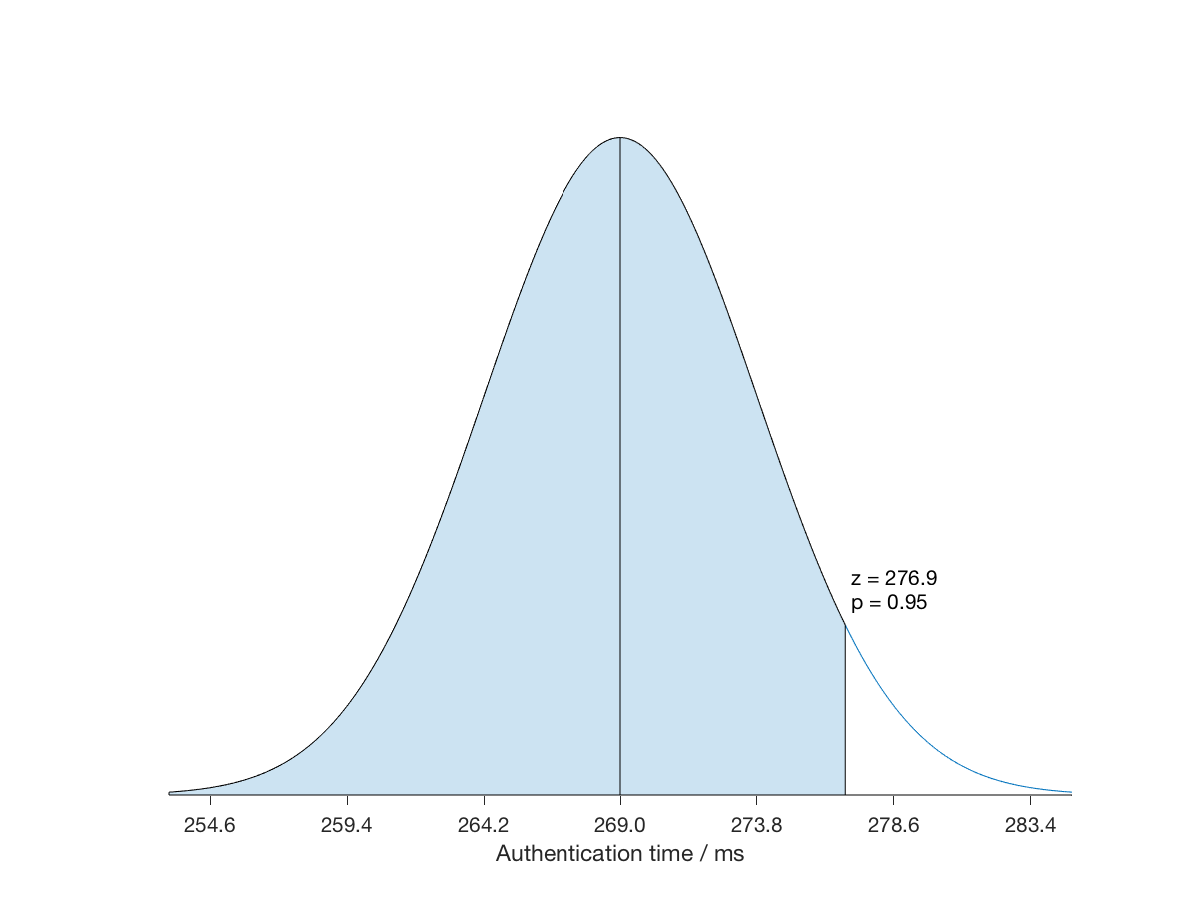
\includegraphics[scale=0.8]{figures/basicauthplot.eps}}
\caption{Histogram of basic authentication protocol runtime ($n = 400$)}
\label{basicauthplot}
\end{figure}

\subsection{Runtime of the mutual authentication protocol}

To three significant figures, the sample mean for the runtime of the mutual authentication protocol was 1.090 s, with a standard deviation of 7.5 ms. \autoref{mutualauthplot} shows a histogram of the recorded timings of the length of the protocol execution.

\begin{figure}[tbh]
\centerline{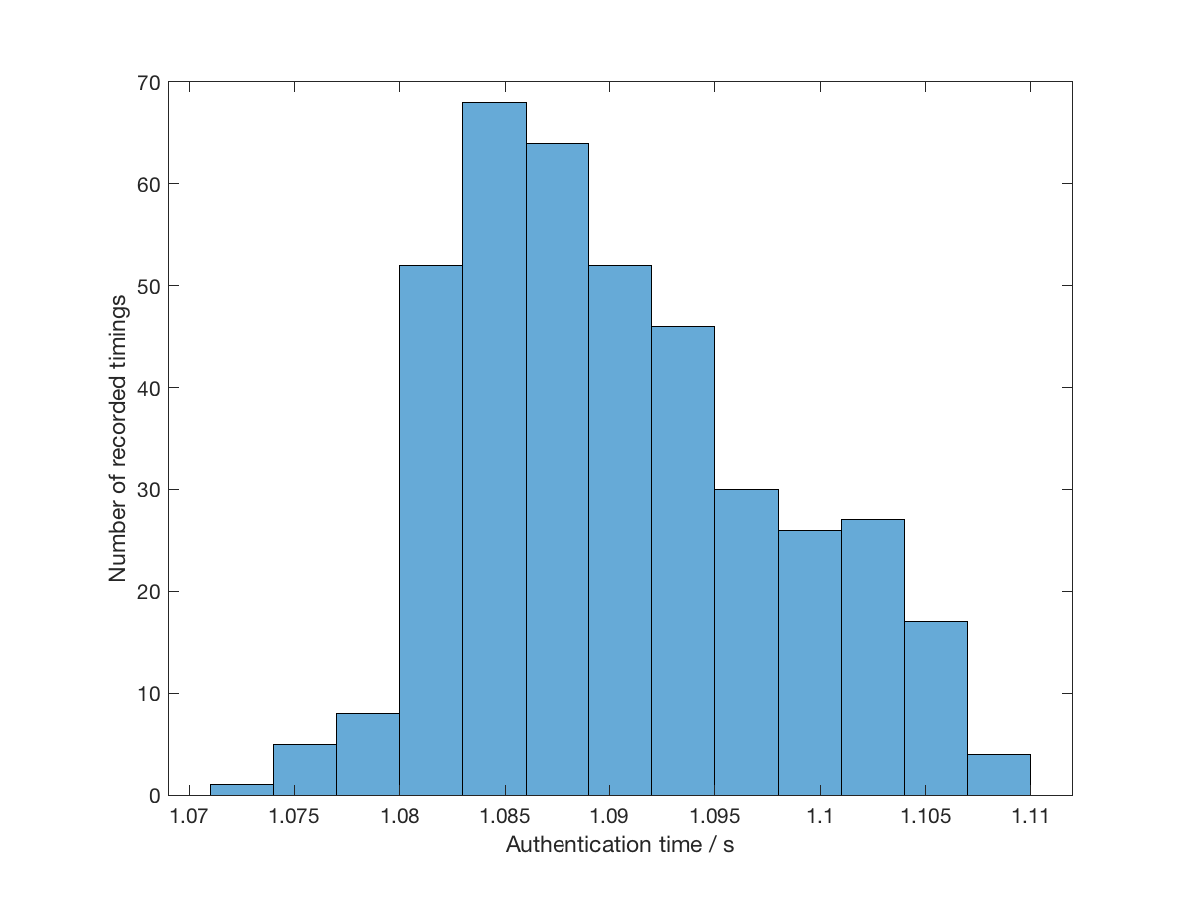
\includegraphics[scale=0.8]{figures/mutualauthplot.eps}}
\caption{Gaussian distribution of mutual authentication protocol runtime}
\label{mutualauthplot}
\end{figure}

We can see clearly that the mutual authentication protocol is significantly slower. This is likely due mostly to two reasons. For one, many more cryptographic operations are performed -- the basic protocol does ECDSA once, whilst the mutual protocol generates an EC key pair, does ECDH and the KDF twice, AES once and CBC-MAC once. Further, I had to implement the concatenation KDF myself, and thus it doesn't have the benefit of hardware acceleration.

\subsection{Comparison to MIFARE Classic authentication protocol runtime}

According to the datasheet of the MIFARE Classic EV1 4k (the card used by the university), authentication should take no longer than roughly 7 ms -- 2 ms to authenticate to a sector on the card, 5 ms to read data, e.g. to fetch CRSID. However, there are many readers around the university that can take up to 2 s to authenticate a card -- this is likely due to the fact that an external database is being queried for the card's access permissions. Therefore, I do not believe that the system utilising either of the protocols described in this dissertation is unusable, by any means.

\section{Security of the protocols}

\subsection{Resistance to replay attacks}

A replay attack is when an adversary eavesdrops on a valid exchange between a real card and reader, and then replays messages sent by, e.g. the reader, in order to trick a real card into believing it's communicating with a real reader, and thus extract sensitive information stored on the card. Alternatively, the attacker may try to replay the card's communications in order to gain access to a restricted location. In practice, this can be done relatively easily by installing some sort of RFID-capable device next to a real reader that stores all overheard communications. The attacker can retrieve this device after some time and analyse the stored exchanges in order to prepare an application capable of performing a replay attack. This application could run on an RFID-capable smartphone, for instance.

A replay attack imitating the card's communications will not work on either of the protocols described in this dissertation. The reason for this is that both protocols utilise some form of cryptographic nonce. Taking the basic protocol as an example, if an attacker attempted to replay a card's response to a reader's request for a nonce signature, the chance that the nonce used in the recorded communication matches the nonce provided during the replay attack attempt are vanishingly small -- the nonce is 100 bytes in length, thus the chance of a nonce match is approximately $10^{-240}$. In a similar way, the mutual authentication protocol uses ephemeral key pairs to prevent replay attacks.

On the other hand, if a replay attack imitates the reader's communications, the basic authentication protocol is vulnerable, in that the card will divulge sensitive information. This is because the card doesn't authenticate the reader, and responds to all requests for a nonce signature with its unencrypted certificate. On the other hand, because the mutual authentication protocol \emph{does} authenticate the reader, an adversary will not be able to decrypt the card's encrypted certificate (referred to as the opaque data). The detailed reasoning for this is described in \autoref{sec:mutualauth}.

\subsection{Resistance to cloning attacks}

As was discussed in \autoref{mifarevulnerabilities}, MIFARE Classic cards have been vulnerable to cloning attacks for nearly a decade. This weakness is the key motivating factor behind the University of Cambridge's desire to replace its current access control system. Thus, it's important that the system described in this dissertation be resistant to such attacks.

Firstly, there's no chance for the card to accidentally divulge its permanent private key, since at no point in the applet's code is the private key used, other than to generate ECDSA signatures or perform ECDH. Therefore, the only attack that could potentially retrieve a card's private key is a side-channel attack. Side-channel attacks aim to take advantage of variations in the the execution time of an algorithm, or the power consumption during execution, as a result of changing stimuli, in order to learn sensitive data, like private keys. This attack would have to target the card's implementation of either ECDSA or ECDH, and thus cannot be avoided by any change to the protocols. The only way to prevent such attacks is to ensure that the chosen model of card implements these algorithms in a time- and power-neutral way.

If we assume that an adversary has somehow managed to obtain a valid card's private key, then this does not immediately mean the system is compromised. Unless the attacker has access to the source code of the authentication protocol applet, they will have to reverse-engineer the operation of the true applet in order to be able to write a clone applet. This is certainly feasible -- consider, for example, the existing clone of CRYPTO-1. However, in order to obtain a card signature, the attacker will need access to a provisioning terminal. If the attacker manages to obtain the provisioning terminal's private key, then they're able to provision cards at will, with whatever access permissions they choose. Thus, in order to keep the system secure, the main concern should be securely storing the provisioning terminal's private key, and restricting access to the physical provisioning terminal.

\subsection{Vulnerability to relay attacks}

Both protocols are vulnerable to what is known as a \emph{relay} attack, a type of man-in-the-middle (MITM) attack. In order to perform such an attack, an adversary must be in possession of two devices that are RFID-capable. Further, these two devices must be able to communicate with one another. One device must be placed within range of a victim's card (device A), and the other must be within range of the target reader (device B). The attack is described in the following paragraph.

By appearing to the target reader to be an RFID tag, B causes the reader to initiate the authentication protocol. B relays all communications sent by the reader to A. When A receives data from B, it relays the data to the victim's card, and thus the card believes it has been engaged in the protocol with a valid reader. When the card responds to the initial command, A relays this response to B, who then relays it to the reader. Because all the cryptographic processing occurred on valid devices, the reader will grant access. Recognise that in order for the attack to work, both relay devices must be within range of their targets at the same time, for the duration of the protocol execution. Thus the conditions for the attack are difficult to achieve.

Relay attacks can be prevented by a distance-bounding protocol, which would allow the reader to establish an upper bound on the physical distance between itself and the card. Such a protocol is based on timing the delay between when the initial authentication command is issued and when the response is received. The delay time enables the reader to compute an upper bound on the distance, by dividing the round-trip delay by twice the speed of light. This computation is based on the fact that electromagnetic waves, such as radio waves that are involved in contactless communication, travel nearly at the speed of light in air, but cannot travel faster. 

\chapter{Conclusion}

The access control system described in this dissertation avoids the mistakes made by the MIFARE Classic system, which were discussed in \autoref{sec:mifareclassic}. It offers two protocols based on asymmetric key cryptography: a basic protocol that authenticates the card's identity, and a more advanced protocol which performs mutual authentication of both the card and reader.

The system utilising the basic protocol is able to perform authentication in at most 276.9 ms, with 95\% confidence, whilst the system utilising the mutual authentication protocol is able to perform authentication in at most 1.103 s, with 95\% confidence.

\section{Achievements}

Two protocols were devised and implemented in two separate applications, one running on the card, the other on the reader. A command-line provisioning application for provisioning and reprogramming cards was written. The system utilising the basic protocol is able to authenticate a card in at most 280 ms, to a high degree of confidence -- well under the requirement of one second. Furthermore, three of the listed extensions were implemented: mutual authentication, untraceability and resilience to cloning.

\section{Lessons learned}

The process of getting to grips with the details of smartcard development was certainly the most difficult part of this project. If this learning curve had not been so steep, I would've perhaps had more time to implement further extensions to the project.

Much was learnt about the considerations specific to developing for memory-impoverished systems. Specifically, the importance of ensuring that different data items must necessarily be stored in different types of memory, in order to ensure efficient execution and to maximise the lifetime of the system.

\section{Further work}

\begin{itemize}
\item Implement the secure messaging capability from the OPACITY-FS protocol.
\item Design and implement a filesystem for the card.
\item Implement persistent binding, as in OPACITY-FS.
\item Implement an attack, as discussed in \cite{opacityanalysis}, targetting the properties of outsider deniability and untraceability, for the protocol featuring persistent binding.
\end{itemize}

%%%%%%%%%%%%%%%%%%%%%%%%%%%%%%%%%%%%%%%%%%%%%%%%%%%%%%%%%%%%%%%%%%%%%
% the bibliography
\addcontentsline{toc}{chapter}{Bibliography}
\bibliography{refs}

%%%%%%%%%%%%%%%%%%%%%%%%%%%%%%%%%%%%%%%%%%%%%%%%%%%%%%%%%%%%%%%%%%%%%
% the appendices
\appendix

\chapter{Project Proposal}
\label{appendix:proposal}

% Note: this file can be compiled on its own, but is also included by
% diss.tex (using the docmute.sty package to ignore the preamble)
\documentclass[12pt,a4paper,twoside]{article}
\usepackage[pdfborder={0 0 0}]{hyperref}
\usepackage[margin=25mm]{geometry}
\usepackage{graphicx}
\usepackage{parskip}
\begin{document}

\begin{center}
\Large
Computer Science Tripos -- Part II -- Project Proposal\\[4mm]
\LARGE
Efficient Asymmetric Cryptography for RFID Access Control\\[4mm]

\large
J.~Fenton, Fitzwilliam College

Originator: Dr M.~Kuhn

11 October 2017
\end{center}

\vspace{5mm}

\textbf{Project Supervisor:} Dr M.~Kuhn

\textbf{Director of Studies:} Dr R.~Harle

\textbf{Project Overseers:} Dr S.~Holden  \& Dr N.~Krishnaswami

% Main document

\section*{Introduction}

The current university access control system is based on the MIFARE Classic smart card, which conforms to ISO 14443 Type A, a standard for contactless integrated circuit cards to communicate with a ``coupling device'' (i.e. a smart card reader) over radio frequency. There are huge numbers of this particular card in existence --- over 200 million are in use today.

The cryptography used in the card, a scheme named CRYPTO-1, was developed in-house by the manufacturer of the MIFARE Classic, NXP Semiconductors. NXP chose to keep the scheme secret, a practice known as security by obscurity. Such practice is eschewed by the security community because naturally, all cryptographic schemes are bound to have weaknesses and if researchers (or others) are not able to analyse a scheme, then they cannot provide advice as to how flaws within said scheme can be fixed. Furthermore, obscurity does not prevent others from deducing the scheme by observing it in operation and indeed this was the case for CRYPTO-1. In December 2007, a presentation at the Chaos Communication Congress (an annual security conference) by two German researchers, Nohl and Pl{\"o}tz, described a partial reverse engineering of CRYPTO-1, as well as some weaknesses. They managed to do this by reconstructing the card's electronic circuit from photos of the chip. They then verified their reconstruction by eavesdropping on the reader-card communication. Just a few months later, in March 2008, researchers in the Digital Security group at Radboud University Nijmegen revealed a complete reverse engineering of the scheme and were able to clone and manipulate the contents of a MIFARE Classic card. The most serious attack they detailed in their paper can recover the card's cryptographic key in under a second using only a laptop, without any pre- computation. NXP tried to obtain an injunction to prevent publication of the paper but were unsuccessful.

Ignoring the fact that the CRYPTO-1 scheme is inherently flawed, NXP's choice to use symmetric key cryptography for the MIFARE Classic was perhaps a misstep. Symmetric ciphers utilize what is called a shared secret, or secret key. Two parties wanting to communicate will first exchange this key over a secure channel and then use it to encrypt/decrypt messages sent between them. In the case of access control cards, this means that a card will store just one key, its own secret key, but that key will be stored in every door reader to which the card has access. This means that if a door reader is compromised, and the attacker is able to retrieve all the keys stored within, then they're able to clone any card which had access to that door. If this door is not in a very specific department, then many people will have access to it, and thus the attacker will have access to a very diverse set of doors --- essentially, the entire system is compromised. Such a weakness does not exist when using a scheme based on asymmetric key cryptography, in which each card has not one but two keys --- one public, one private. The private key is known only to the owner and is never sent over any channel, whilst the public key is known to everyone. If two parties wish to communicate, then they encrypt their messages with each other's public keys. The message can now only be decrypted with the recipient's private key, which only the recipient knows. In this case, the door reader contains only a long list of public keys corresponding to all the cards that can access the door. Thus, an attacker who's able to compromise a reader doesn't learn any secret information except for the door's private key. This only allows them to clone that specific door reader and doesn't compromise any other cards or readers in the system.

The aim of the project is to produce an access control system that uses asymmetric key cryptography to authenticate smart cards. The system should act as a replacement for the existing MIFARE Classic system.

\section*{Starting point}

The project will make significant use of the material from Security I and Security II --- I have already studied the lecture notes for Security II, although I have set aside some time in my plan for recap. Further, material from Object-Oriented Programming and Further Java will be utilised when writing the smart card application, which runs on the JavaCard platform and supports a subset of the Java language.

A previous attempt was made at this project by Denys Natykan, and so his dissertation must be mentioned as a starting point. However, I already anticipate significant differences between our end products as I intend to use a rather different authentication protocol.

\section*{Substance and structure of the project}

The objective of the project is to produce an access control system that implements an authentication protocol based on asymmetric key cryptography. As well as producing a card application and reader application that implement the authentication protocol, I intend to write a card-provisioning application that can be used to issue new cards or reprogram existing cards.

I intend to compare at least two different digital signature algorithms (DSAs) for speed in my evaluation, and it's possible that one or more of these algorithms won't be implemented by the JavaCard SDK, in which case I will have to implement them myself.

Given that smart cards are low power, I expect that I may have to spend time optimising the protocol, so that authentication happens within the required time.

\section*{Success citeria and evaluation}

\begin{itemize}
\item An authentication protocol must be chosen.
\item The protocol must be implemented in two separate applications --- one
to run on the card, the other on the reader.
\item A command-line application must be written for provisioning and
reprogramming cards.
\item The system must be able to authenticate a card in less than one second.
\item The system should be tested to ensure it operates as the protocol dictates it should.
\item The dissertation must be planned and written.
\end{itemize}

\section*{Possible extensions}

\begin{itemize}
\item Mutual authentication of both card and controller so that only authorised readers (i.e. university door controllers) are able to communicate with cards.
\item Provide user untraceability as a feature of the authentication protocol.
\item Ensure the system is resilient to cloning.
\item Implement a GUI for the card-issuing application.
\end{itemize}

\section*{Timetable}

\subsection*{Weeks 1 to 2}

Initial research period. I will familiarise myself with existing authentication protocols and either select one of them to use, either in full or as a guideline, else I will design one myself. Familiarisation with the JavaCard SDK and the GlobalPlatform API.

\subsection*{Weeks 3 to 4}

Implement a very basic challenge-response application on the smart card. Gain a deeper understanding of the J3A040 smart card, specifically the memory structure and the implications of this for fast authentication.

\subsection*{Weeks 5 to 10}

Implement the chosen authentication protocol on the card and reader. Implement the card-provisioning application to run on computer.

\subsection*{Weeks 11 to 12}

Time reserved for testing the system and sorting out any leftover bugs in the system.

\subsection*{Weeks 13 to 16}

Reserved for dealing with bugs. If the base system is in good working order, then this time can be used to implement extensions. I'm currently undecided as to which extensions will be prioritised --- my choice will depend on available time.

\subsection*{Weeks 17 to 20}

Perform evaluation of the system. Begin writing dissertation.

\subsection*{Weeks 21 to 23}

Time reserved for handling any bugs that escaped notice earlier in the process. This time can be used for writing the dissertation if there's nothing to be fixed.

\subsection*{Weeks 24 to 25}

Finish writing initial draft of the dissertation.

\subsection*{Weeks 26 to 28}

Time left to send dissertation draft to supervisor for review (this may happen a couple of times) and make changes. Finalise dissertation and submit electronically.

\section*{Resources declaration}

\begin{itemize}
\item NXP J3A040 --- a programmable smart card supporting JavaCard SDK and GlobalPlatform API.
\item SCL3711 --- a USB smart card reader.
\item JavaCard SDK and GPShell for programming smart cards.
\item My own MacBook Pro and Lenovo Yoga 2 Pro for writing applications,
documentation and dissertation. I plan to use Git for source control, and will regularly push to a remote Bitbucket repository to avoid significant loss in the event that I experience a hard drive failure.
\end{itemize}

\end{document}

\chapter{Card Application Build File}
\label{appendix:cardappbuildfile}

\begin{minted}[breaklines=true]{xml}
<?xml version="1.0"?>
<project name="opacity_fs_impl">
  <taskdef name="javacard" classname="pro.javacard.ant.JavaCard" classpath="ant-javacard.jar"/>

  <target name="jc">
    <javacard>
      <cap jckit="/Users/jacobfenton/Desktop/piiproj/java_card_kit-2_2_2" version="1.0" aid="f234123456101000" output="opacity_fs_impl.cap" sources="/Users/jacobfenton/Desktop/piiproj/opacity_fs_impl/src/
      main/java/org/bitbucket/jfent/opacity_fs_impl">
        <applet class="org.bitbucket.jfent.opacity_fs_impl.OpacityForwardSecrecy ImplementationApplet" aid="f23412345610100001"/>
      </cap>
    </javacard>
  </target>

  <target name="clean">
      <delete dir="./build"/>
  </target>

  <target name="compile">
      <mkdir dir="./build/classes"/>
      <javac srcdir="./src/main/java" destdir="./build/classes">
          <classpath>
              <pathelement path="./lib/api.jar"/>
          </classpath>
      </javac>
  </target>

  <target name="jar">
      <mkdir dir="./build/jar"/>
      <jar destfile="./build/jar/opacity_fs_impl.jar" basedir="./build/classes">
          <zipgroupfileset dir="./lib" includes="*.jar" />
      </jar>
  </target>
</project>
\end{minted}

\end{document}
